\documentclass[11pt]{beamer}
\usecolortheme{beaver}
\usetheme{Madrid}
\usefonttheme{serif} 
\usepackage{amsmath, amssymb, graphicx, booktabs}
\usepackage{siunitx}
\usepackage{bm}
\usepackage{multirow}
\usepackage{caption}
\usepackage{mathptmx}
\captionsetup[figure]{font=scriptsize,labelfont=bf}


\title[Ordinal Pattern Analysis of Time Series]{Feature-Based Clustering of Time Series \\ Using Ordinal Pattern Analysis}
\author[M. H. M. R. S. Dilhani et al.]{
	M.\ H.\ M.\ R.\ S.\ Dilhani\inst{1} \\
	Alejandro C.\ Frery\inst{1} \\
	Andrea A.\ Rey\inst{2}}
\institute[Victoria University of Wellington]{
	\inst{1}School of Mathematics and Statistics, Victoria University of Wellington, New Zealand\\
	\inst{2}LIDEC, Universidad Nacional de Hurlingham (UNAHUR), Argentina}
\date{\today}

\setbeamertemplate{footline}{
	\leavevmode
	\hbox{%
		\begin{beamercolorbox}[wd=.85\paperwidth,ht=2.5ex,dp=1ex,left]{author in head/foot}
			\usebeamerfont{author in head/foot}\hspace{1em} Time Series Analysis Using Ordinal Patterns
		\end{beamercolorbox}%
		\begin{beamercolorbox}[wd=.15\paperwidth,ht=2.5ex,dp=1ex,right]{date in head/foot}
			\usebeamerfont{date in head/foot}\insertframenumber{} / \inserttotalframenumber\hspace{1em}
		\end{beamercolorbox}%
	}
	\vskip0pt
}

\begin{document}
	%===========================================================
	\begin{frame}
		\titlepage
	\end{frame}
	
	%------------------------------------------------
	\begin{frame}{Outline}
		\tableofcontents
	\end{frame}
	
	%===========================================================
	
	\begin{frame}{Motivation and Background}
		\small
		\begin{itemize}
			\item Time series clustering is challenging, especially under stochastic or nonlinear dynamics.
			
			\item \alert{Ordinal patterns} capture the order relations among consecutive data points.
			
			\item \textbf{Bandt \& Pompe (2002)}~\cite{PhysRevLett.88.174102}: introduced \textbf{Permutation Entropy} by mapping time series into ordinal patterns.
			
			\item \textbf{Limitation:} Entropy quantifies disorder but cannot distinguish random from structured dynamics.
			
			\item \textbf{Extension:} \textbf{López-Ruiz et al. (1995)}~\cite{lopez1995statistical} and \textbf{Lamberti et al. (2004)}~\cite{lamberti2004intensive}, introduced \alert{disequilibrium} and \textbf{Statistical Complexity} as complementary measures.
			
			\item The \textbf{Entropy–Complexity Plane} maps time series by entropy $(H)$ and complexity $(C)$, revealing distinct dynamical regimes.
			
			\item \textbf{Goal:} Differentiate \textbf{AR}, \textbf{MA}, and \textbf{ARMA} models using these measures.
		\end{itemize}
	\end{frame}
	
	%-----------------------------------------------------%
	\begin{frame}{From Time Series to Ordinal Patterns: An Example}
		\small
		\begin{itemize}
			\item \textbf{Example:} Mean monthly humidity in Wellington.
			\item Original time series:
			\[
			77.3,\ 81.0,\ 82.4,\ 81.7,\ 83.6,\ 85.6,\ \dots
			\]
		\end{itemize}
		
		\begin{figure}[hbt]
			\centering
			
\includegraphics[width=0.5\textwidth]{humidity graph} 
			\caption{Mean monthly humidity in Wellington}
			\label{fig:humidity}
		\end{figure}
	\end{frame}
	
	%-----------------------------------------------------%
	\begin{frame}{Transforming into Ordinal Patterns}
		\small
		\begin{itemize}
			\item Choose embedding dimension $D = 3$.
			\item Slide a window of size $D$ across the series:
		\end{itemize}
		
		\[
		(77.3, 81.0, 82.4) \rightarrow (1,2,3) = \pi_1
		\]
		\[
		(81.0, 82.4, 81.7) \rightarrow (1,3,2) = \pi_2
		\]
		
		\begin{itemize}
			\item Continue for all overlapping windows ($n - D + 1$ total).
			\item Each window represents an \alert{ordinal pattern} describing local order relations.
		\end{itemize}
		
		\begin{center}
			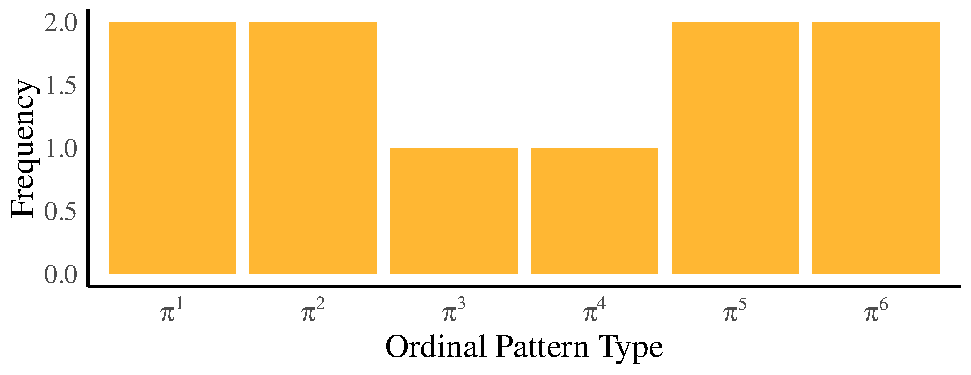
\includegraphics[width=0.5\textwidth]{frequency histogram} 
		\end{center}
	\end{frame}
	
	%-----------------------------------------------------%
	\begin{frame}
	 
		\begin{block}{Definition: Permutation Entropy ($H$)}
			\[
			H(\mathbf{p}) = -\dfrac{1}{\log k} \sum_{i=1}^{k} p(\pi^i) \log p(\pi^i),
			\]
			where $k=D!$ and $p(\pi^i)$ is the proportion of pattern $\pi^i$.
		\end{block}
		
		\begin{block}{Definition: Jensen-Shannon Distance}
			Given a histogram $\mathbf{p}$ and the reference uniform distribution $\mathbf{u} = (1/k, \ldots, 1/k)$ ($k = D!$), the disequilibrium is calculated as:
			\[
			Q'(\mathbf{p},\mathbf{u}) = \sum_{\ell=1}^k \Big( p_\ell \log\frac{p_\ell}{u_\ell} + u_\ell \log\frac{u_\ell}{p_\ell} \Big).
			\]
		\end{block}		
		
		\begin{block}{Definition: Statistical Complexity $C$ }
			\[
			C = H Q
			\]
			where $H$ is normalized entropy and $Q$ is normalized disequilibrium.
		\end{block}
	\end{frame}
		
	%-----------------------------------------------------%
	\begin{frame}
		Conceptual Framework
		\begin{columns}
			\column{0.55\textwidth}
			\begin{itemize}
				\item Transform time series $\{x_t\}$ into \textbf{ordinal patterns}.
				\item Compute:
				\begin{itemize}
					\item Permutation Entropy
					\item Statistical Complexity
					\item Confidence Interval for permutation entropy and complexity
				\end{itemize}
				\item Plot in the \textbf{Entropy–Complexity ($H \times C$)} plane.
				\item Use cluster formation to discriminate models.
			\end{itemize}
			\column{0.45\textwidth}
			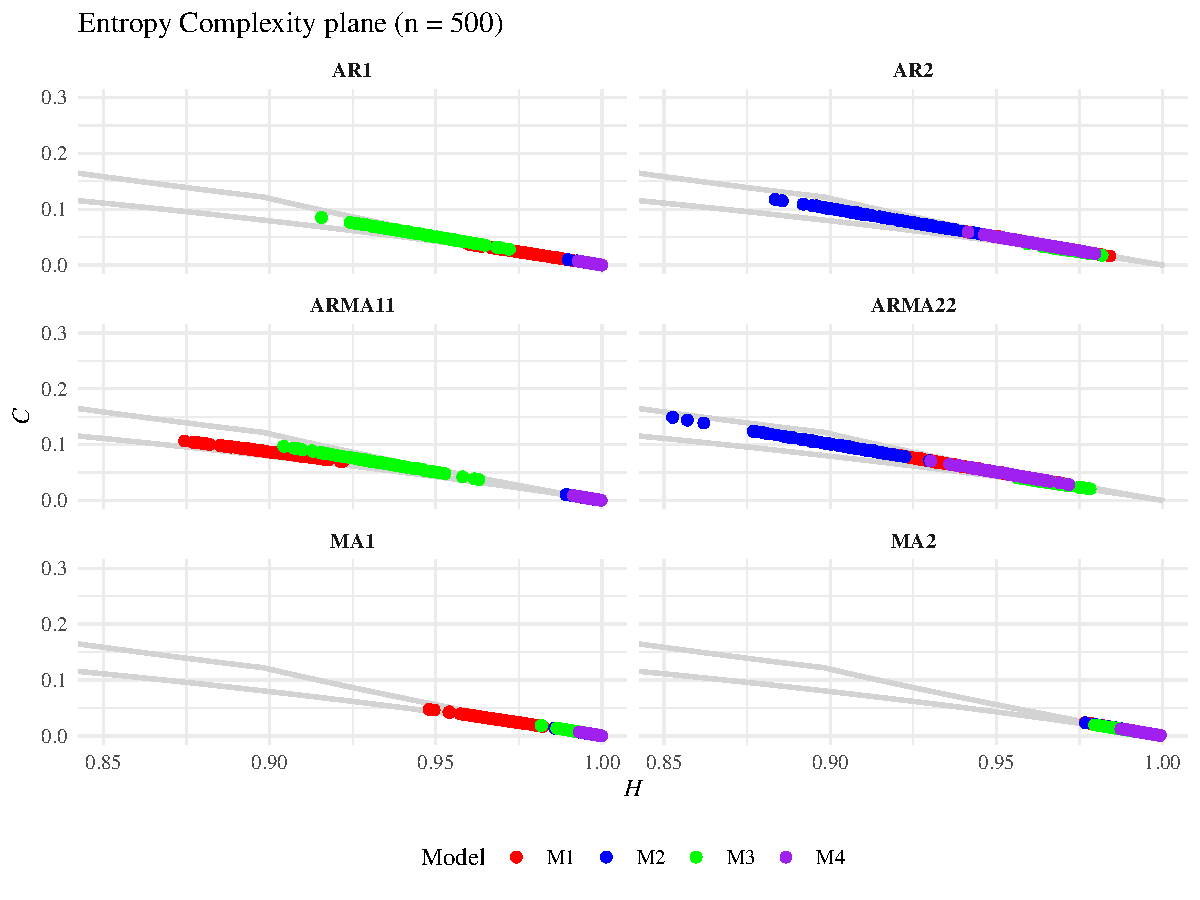
\includegraphics[width=\linewidth]{New_model_group_plot_n500}
			\captionof{figure}{ Entropy–Complexity plane for Sample size $n=500$.}
		\end{columns}
	\end{frame}
	
	%===========================================================
	\section{Methodology}
	\begin{frame}{Experimental Design}
		\begin{itemize}
			\item Models studied:
			\begin{itemize}
				\item $\mathrm{AR}(1)$, $\mathrm{AR}(2)$, $\mathrm{MA}(1)$,  $\mathrm{MA}(2)$, $\mathrm{ARMA}(1,1)$, $\mathrm{ARMA}(2,2)$
			\end{itemize}
			\item Each model simulated with 100 independent replications.
			\item Parameter sets chosen to ensure stationarity and invertibility.
			\item Series lengths: $n = 500, 1000$.
		\end{itemize}
	\end{frame}
	
	%-----------------------------------------------------%
	\begin{frame}{Model Parameter Structure}
		\centering
		\scriptsize
		\begin{tabular}{llrrrr}
			\toprule
			Type & Model & $\alpha_1$ & $\alpha_2$ & $\beta_1$ & $\beta_2$ \\
			\midrule
			$\mathrm{AR}(1)$ & $\mathrm{AR}(1)_{\textrm{M}_1}$ & $0.8$ &  &  & \\
			& $\mathrm{AR}(1)_{\textrm{M}_2}$ & $0.1$ &  &  & \\
			$\mathrm{MA}(1)$ & $\mathrm{MA}(1)_{\textrm{M}_1}$ &  &  & $0.8$ & \\
			& $\mathrm{MA}(1)_{\textrm{M}_2}$ &  &  & $0.1$ & \\
			$\mathrm{ARMA}(1,1)$ & $\mathrm{ARMA}(1,1)_{\textrm{M}_1}$ & $0.8$ &  & $0.8$ & \\
			& $\mathrm{ARMA}(1,1)_{\textrm{M}_2}$ & $0.1$ &  & $0.1$ & \\
			\bottomrule
		\end{tabular}
		\captionof{table}{Example of parameter sets ensuring diversity.}
	\end{frame}
	
	%-----------------------------------------------------%
	\begin{frame}
			Feature Extraction and Central Points
		\begin{columns}
		\column{0.55\textwidth}
		\begin{itemize}
				\item For each realization, compute:
			\begin{itemize}
				\item Entropy (\(H\)) — randomness
				\item Complexity (\(C\)) — structure
				\item Confidence Interval(CI) for $H$ and $C$
			\end{itemize}
			\item For each model, identify the \textbf{central (median) point} $(H^*, C^*)$ using PCA projection.
			\item Median ensures the point is the most representative of the model’s behavior, as referred to in Chagas et al.~\cite{Chagas2022a}. 
		\end{itemize}
		\column{0.45\textwidth}
		
\includegraphics[width=\linewidth]{Median_HC_Shannon_Entropy_case1.pdf}
		\captionof{figure}{Example of central $(H^*, C^*)$ points.}
	    \end{columns}
	\end{frame}
	
	%===========================================================
	\section{Results: Case-Based Analysis}
	\begin{frame}{Case Study Design}
		\begin{itemize}
			\item \textbf{Case 1–3:} Positive, negative, and mixed-sign coefficients.
			\item \textbf{Case 4–6:} Extended experiments with selected extreme and central ARMA models.
			\item Two sample size: $n=500, n=1000$.
			\item Each case analyzed using:
			\begin{itemize}
				\item The density of points in the $H \times C$
				\item Scatter plots with confidence intervals for $H$ and $C$ 
				%\item Heat maps for model classification
			\end{itemize}
		\end{itemize}
	\end{frame}

     %-----------------------------------------------------% 	
	%\begin{frame}{Case 1 — Positive Coefficients}
	%	\centering
	%	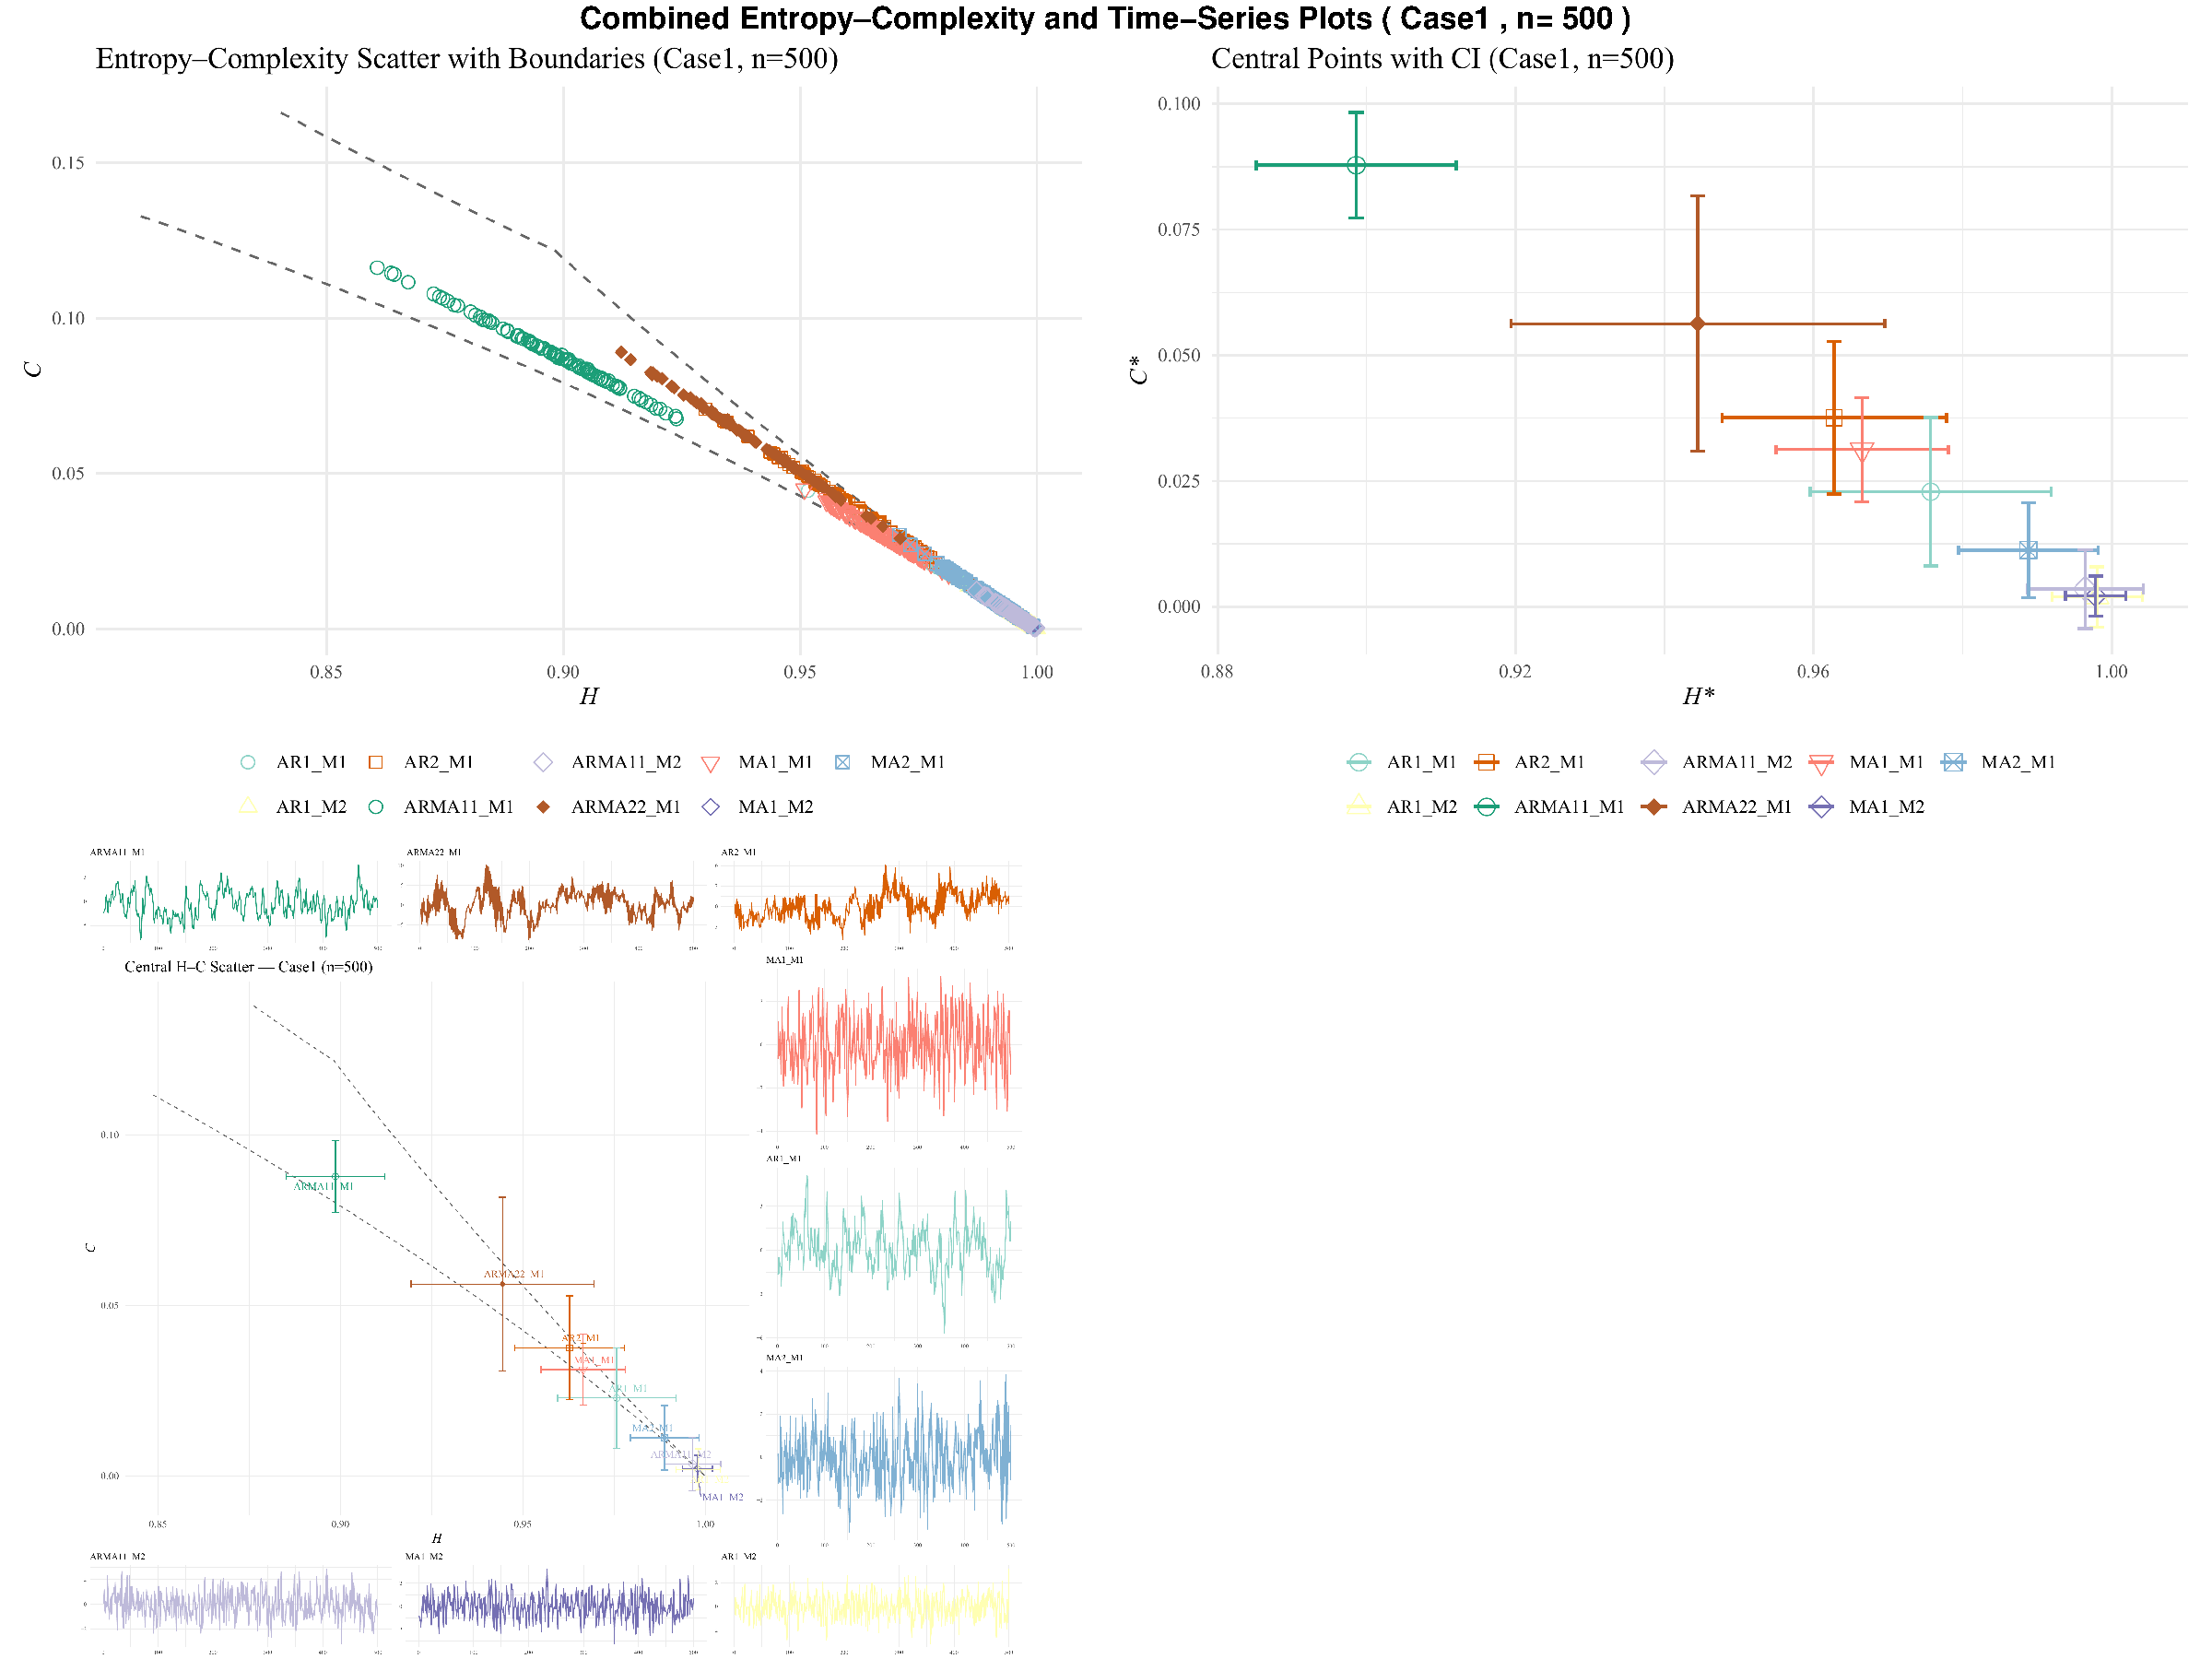
\includegraphics[width=0.7\textwidth]{Combined3Plots_Case1_n500.pdf}
	%	\captionof{figure}{Entropy–complexity scatter plot and associated time series ($n=500$) for positive model coefficients.}
	%\end{frame}
	
		\begin{frame}{Case 1 — Positive Coefficients}
		\centering
		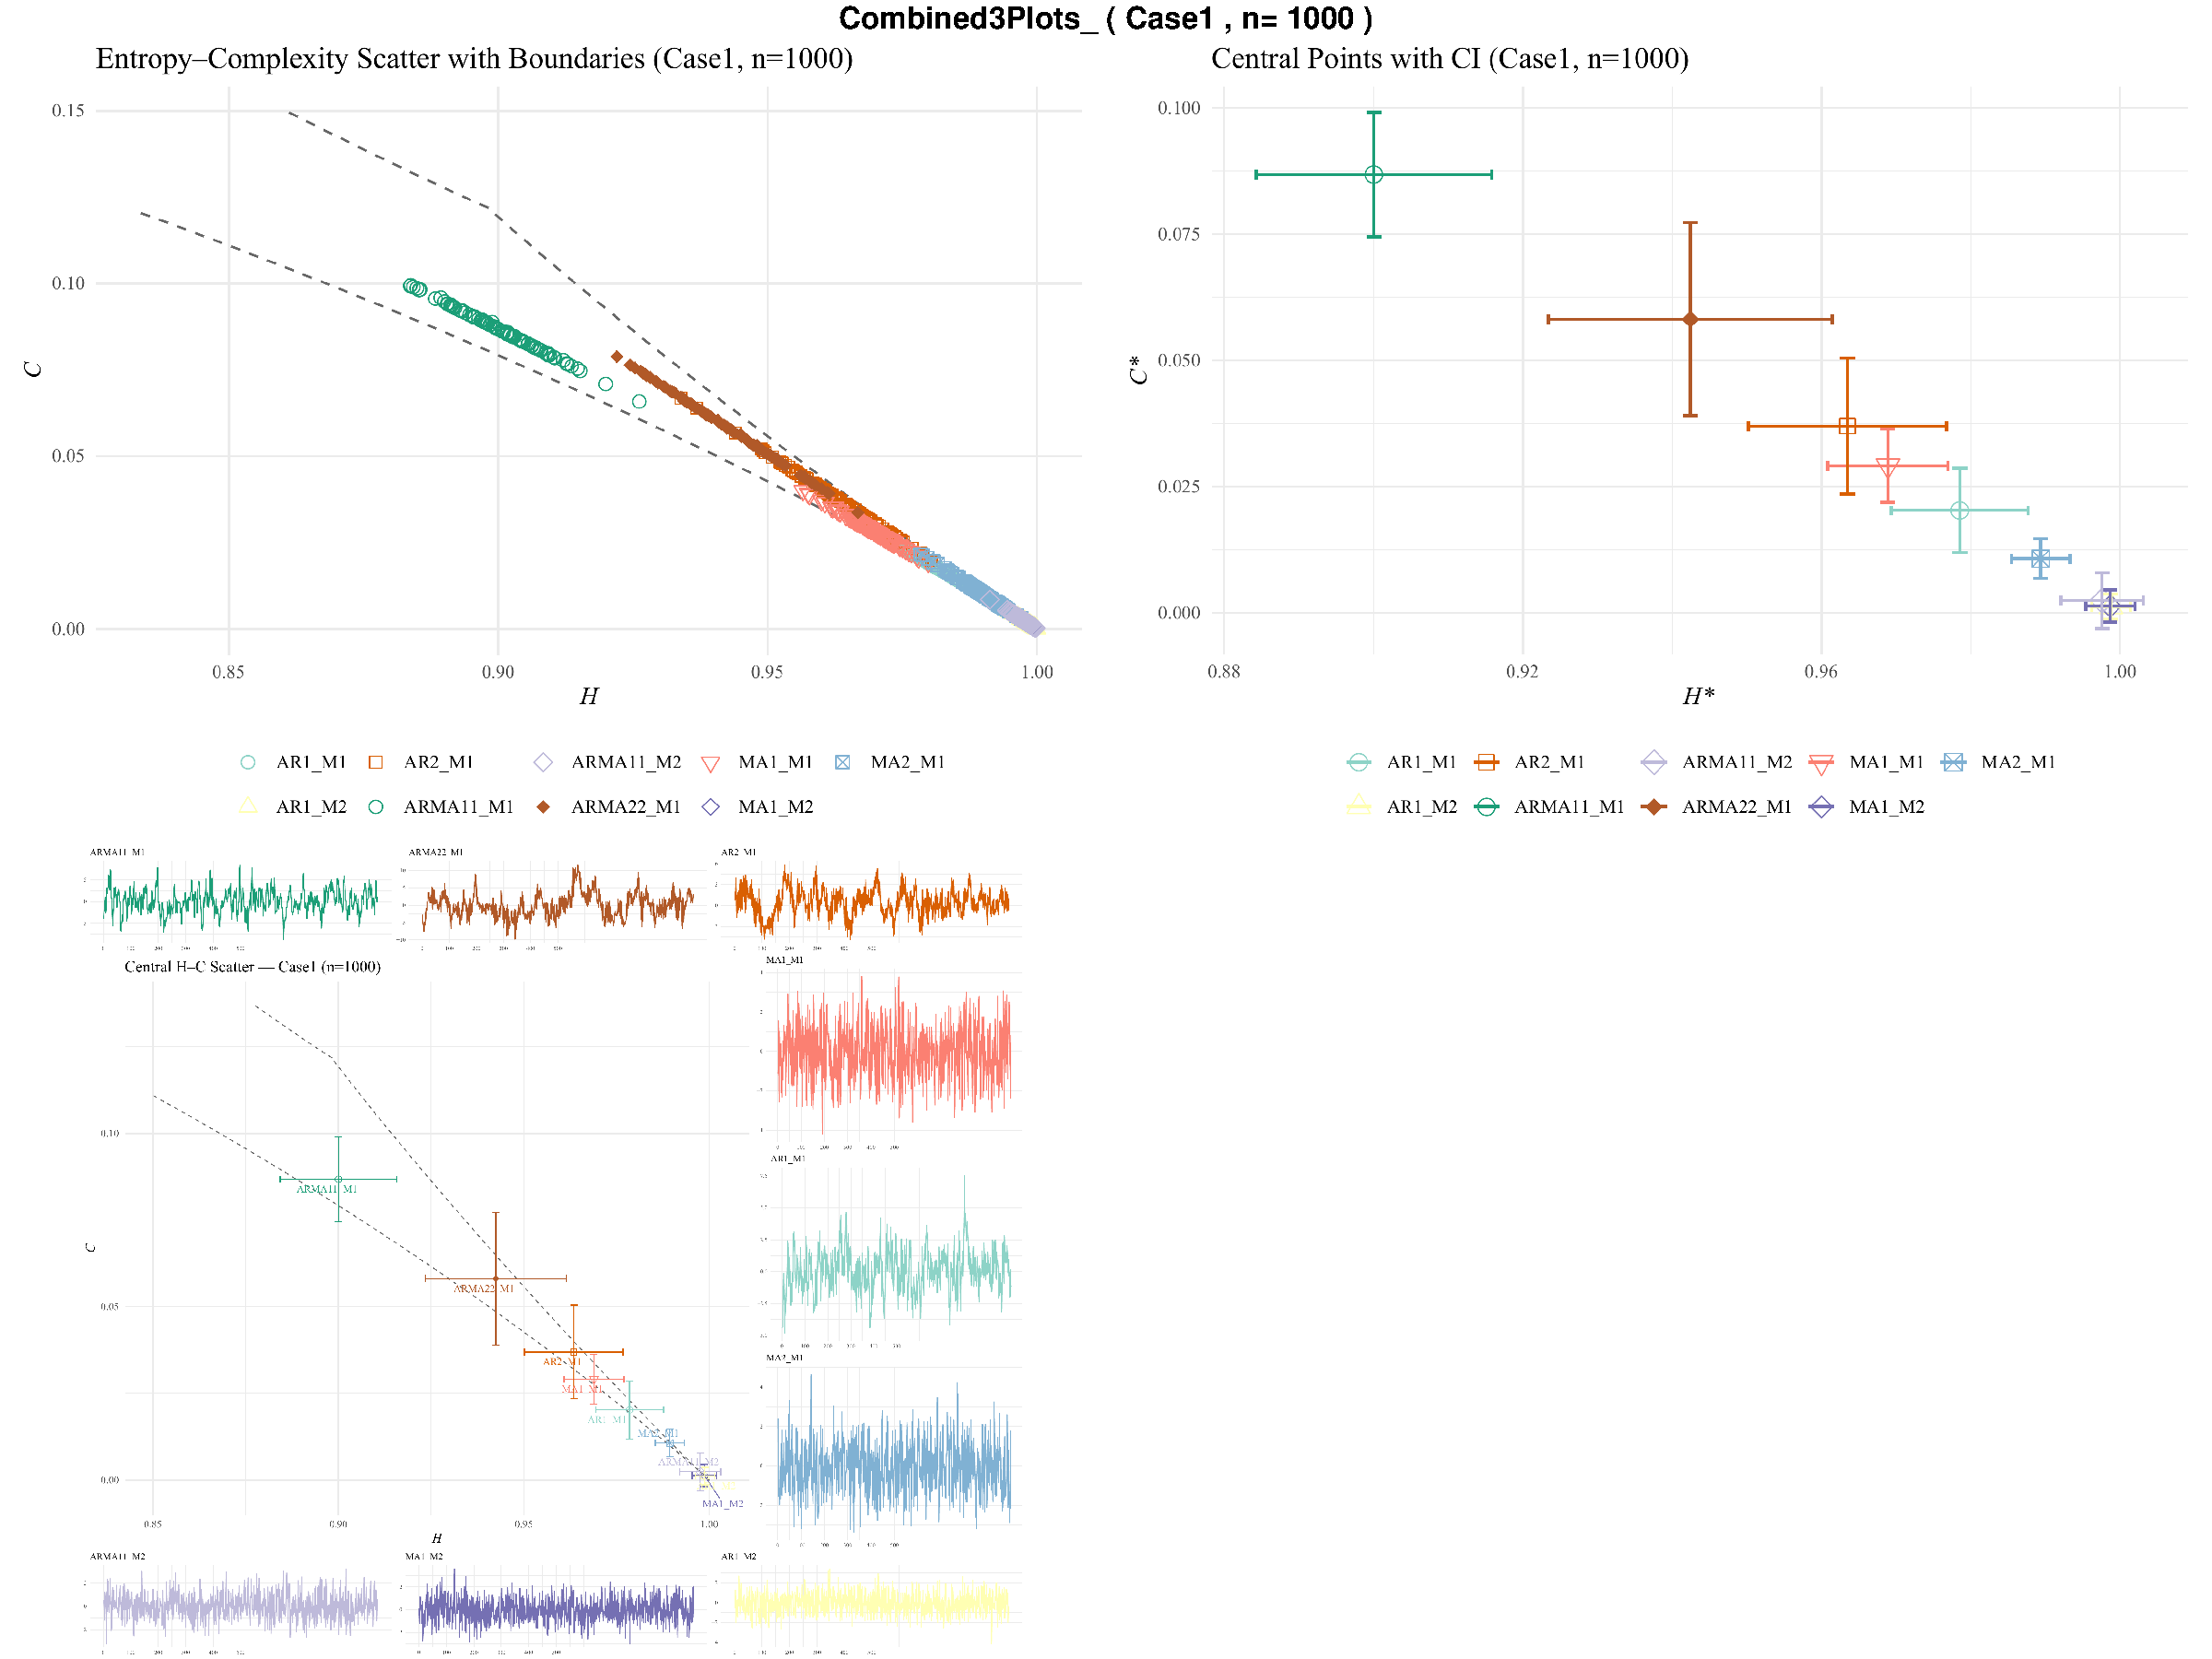
\includegraphics[width=0.7\textwidth]{Combined3Plots_Case1_n1000.pdf}
		\captionof{figure}{Entropy–complexity scatter plot and associated time series ($n=1000$) for positive model coefficients.}
	\end{frame}
	
	\begin{frame}{Case 2 — Negative Coefficients}
		\centering
		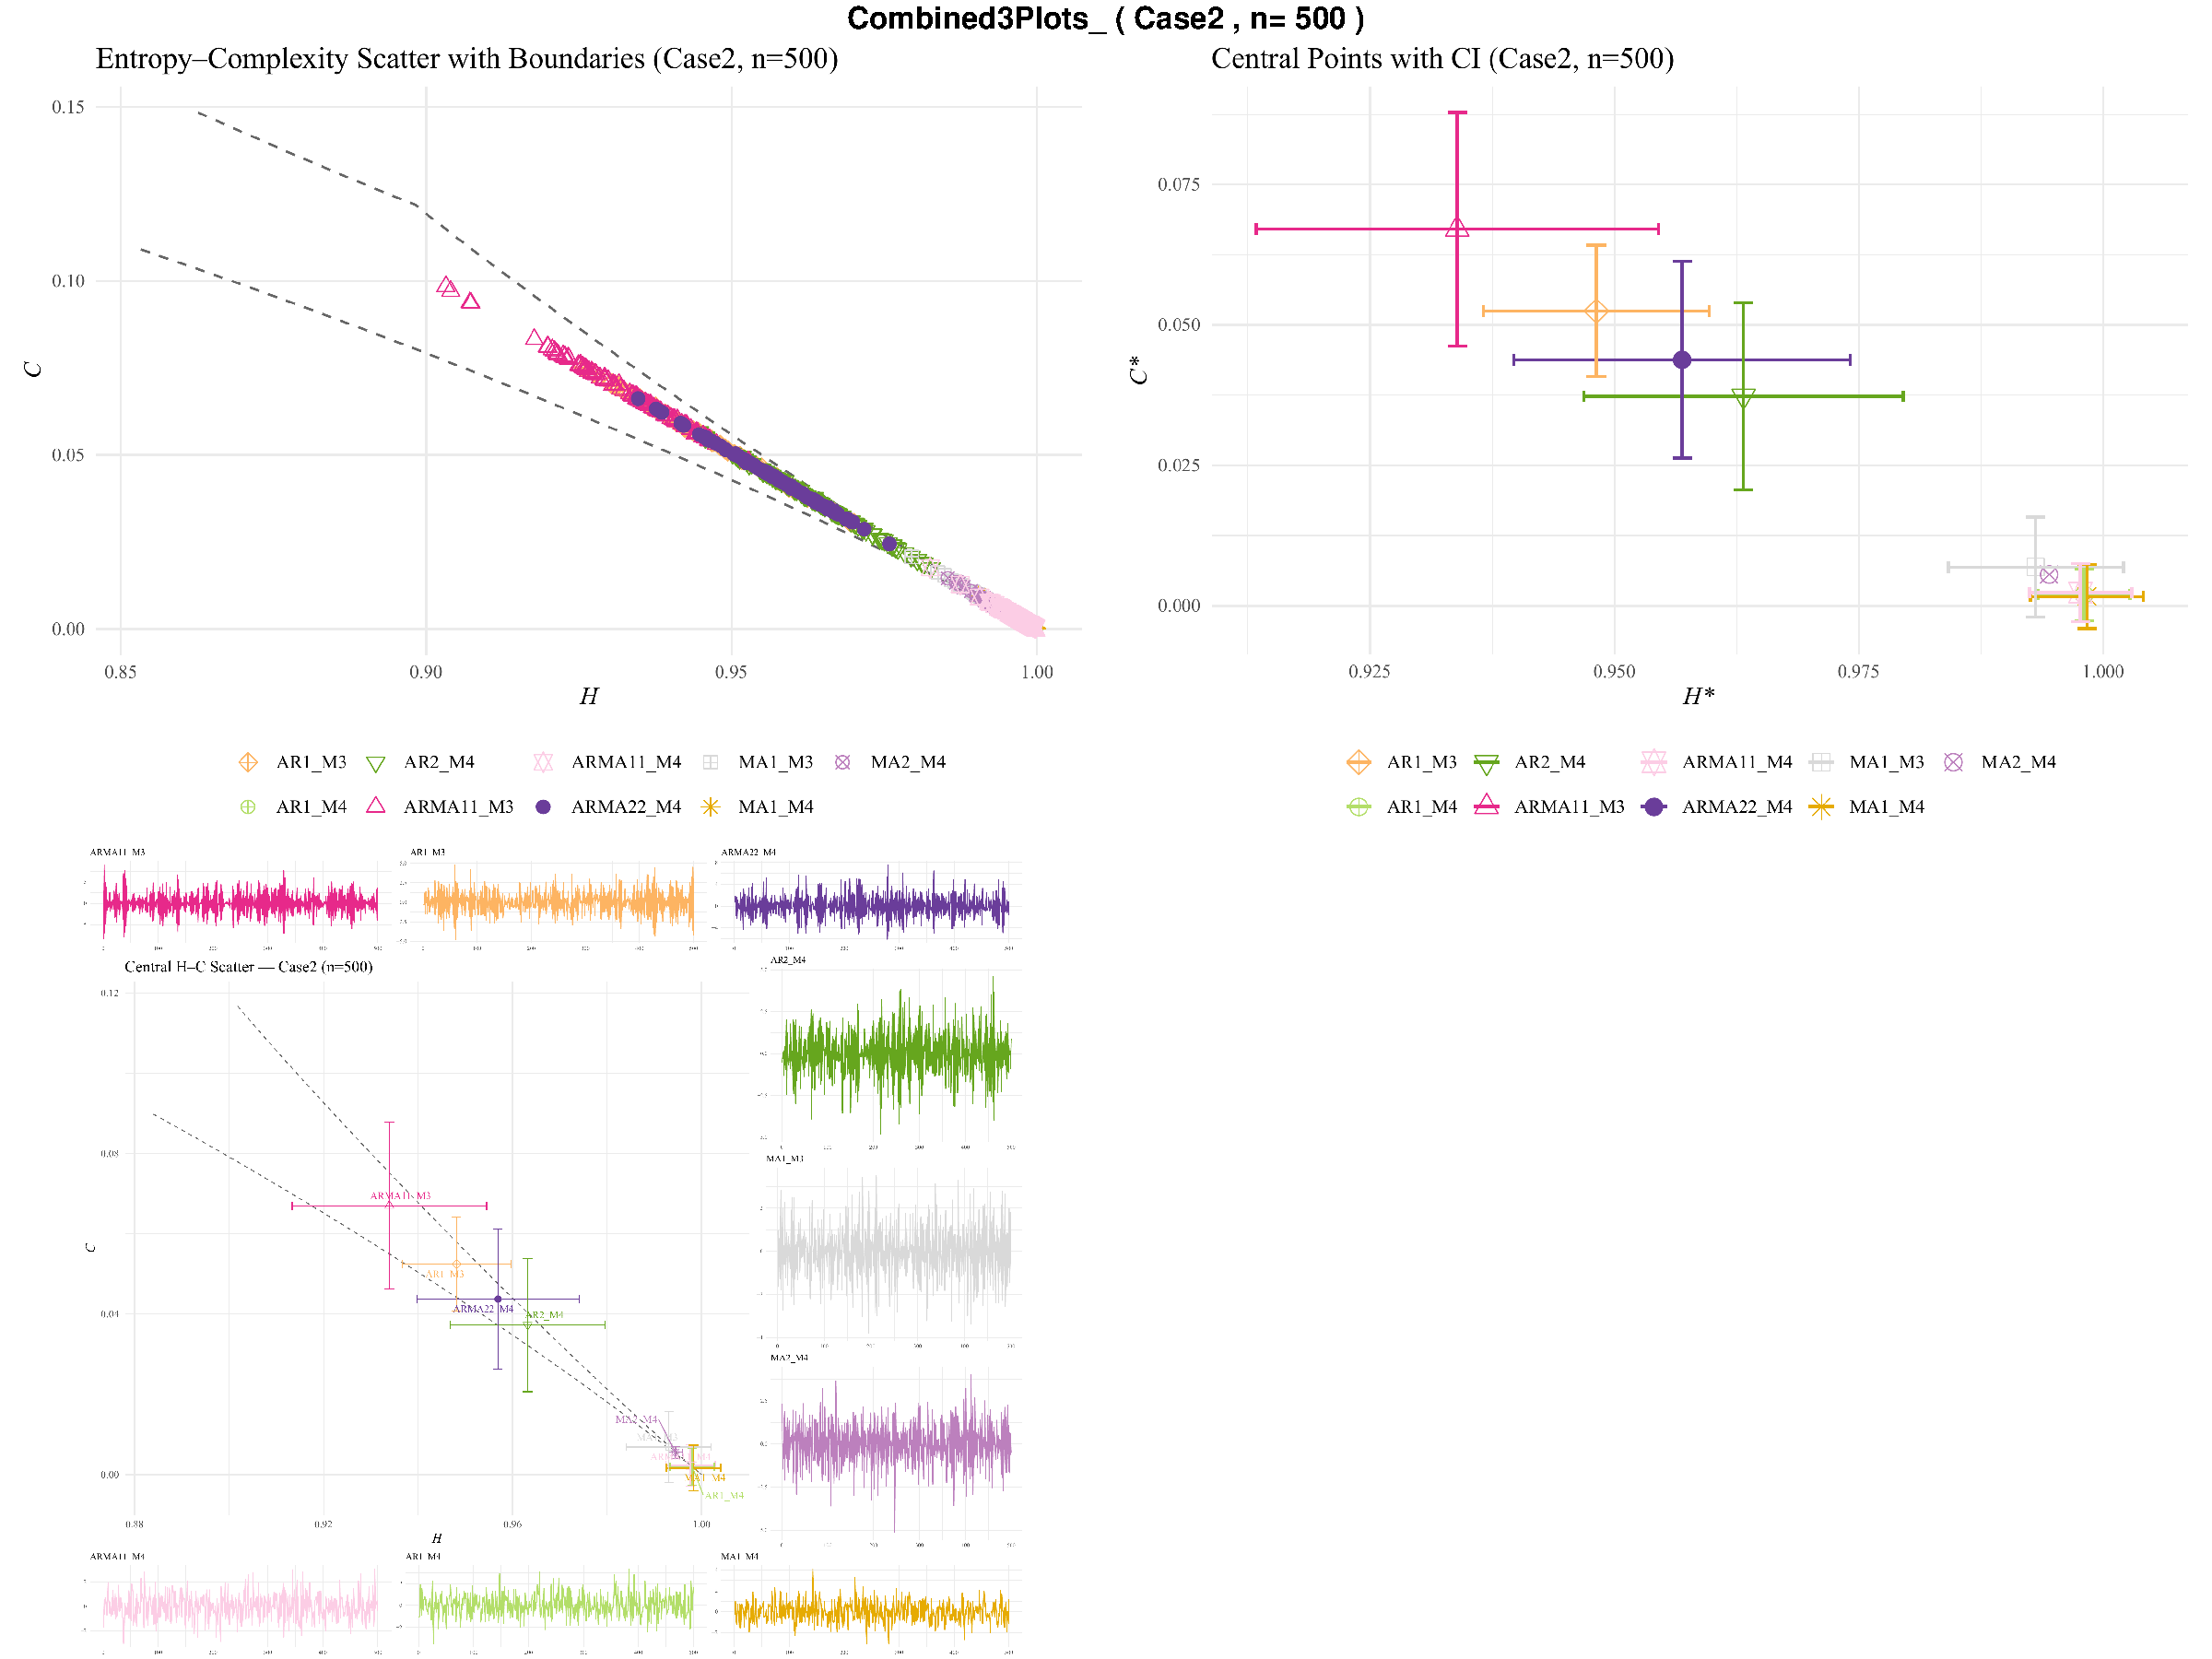
\includegraphics[width=0.7\textwidth]{Combined3Plots_Case2_n500.pdf}
		\captionof{figure}{Entropy–complexity scatter plot and associated time series ($n=500$) for  negative parameters.}
	\end{frame}
	
	\begin{frame}{Case 2 — Negative Coefficients}
		\centering
		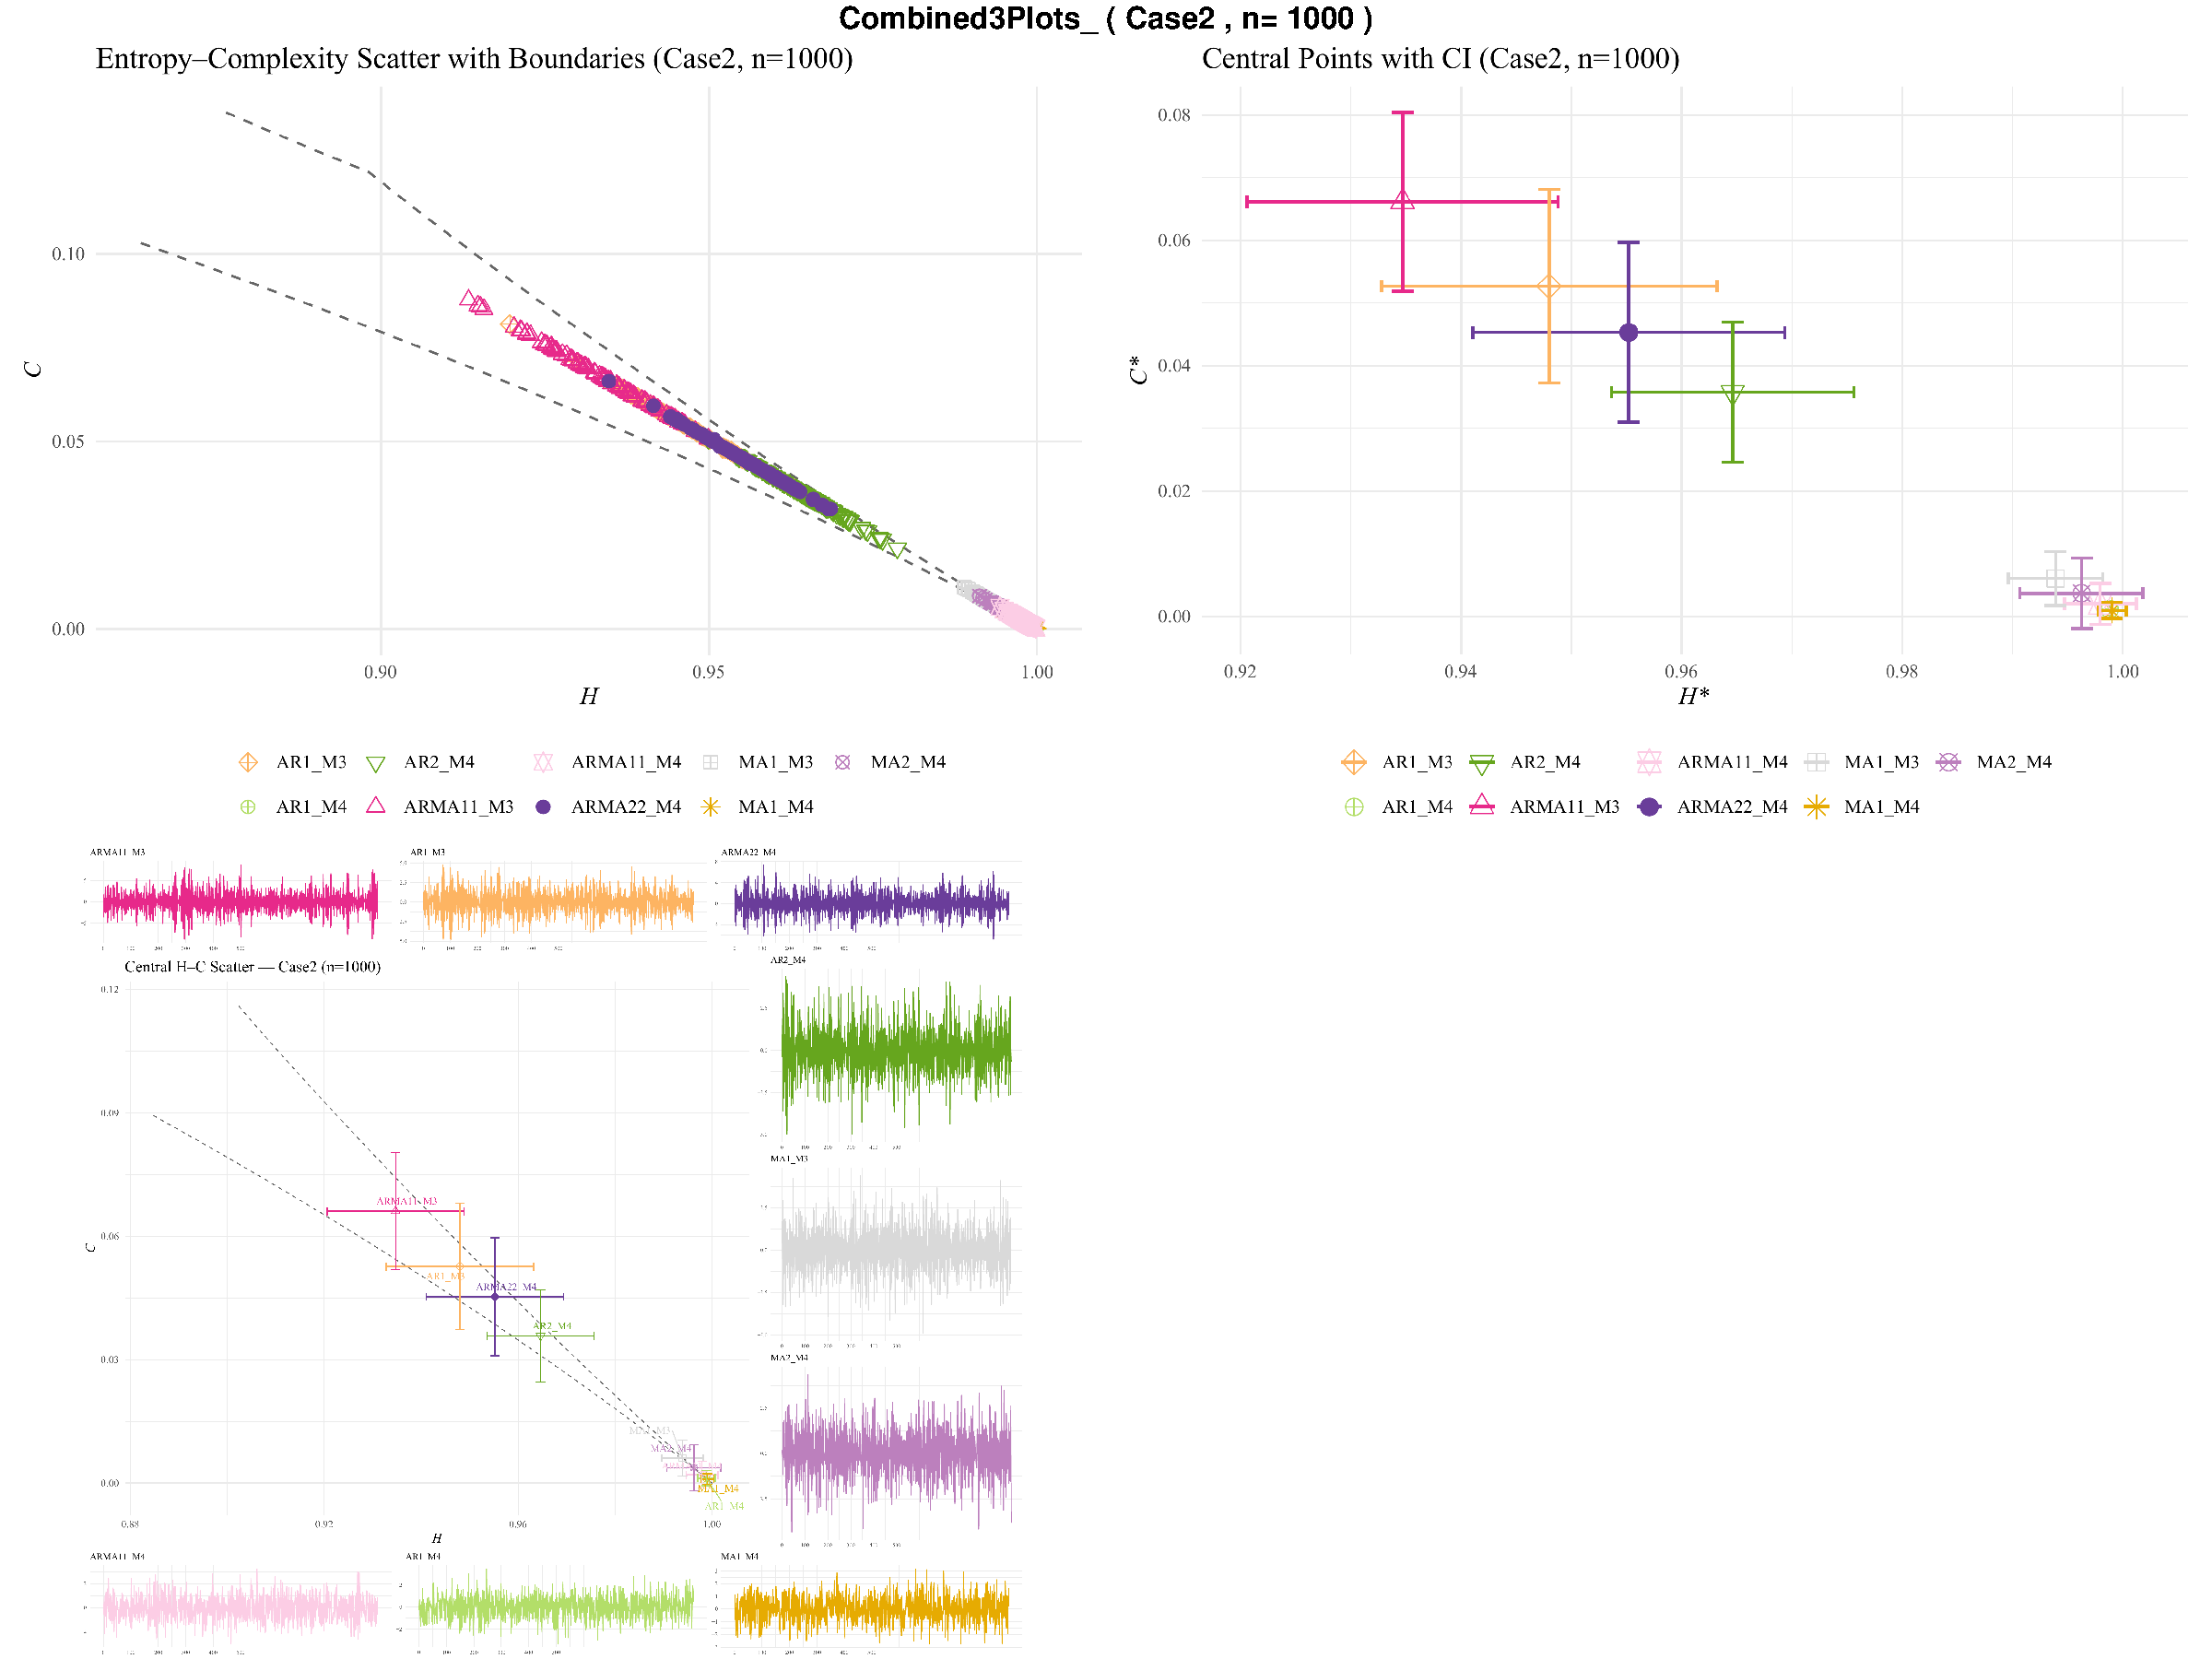
\includegraphics[width=0.7\textwidth]{Combined3Plots_Case2_n1000.pdf}
		\captionof{figure}{Entropy–complexity scatter plot and associated time series ($n=1000$) for  negative parameters.}
	\end{frame}
	
	%-----------------------------------------------------%
\begin{frame}{Case 3 — Mixed-Sign Coefficients}
	\begin{columns}[c] % 'c' centers content vertically
		\column{0.48\textwidth}
		\centering
		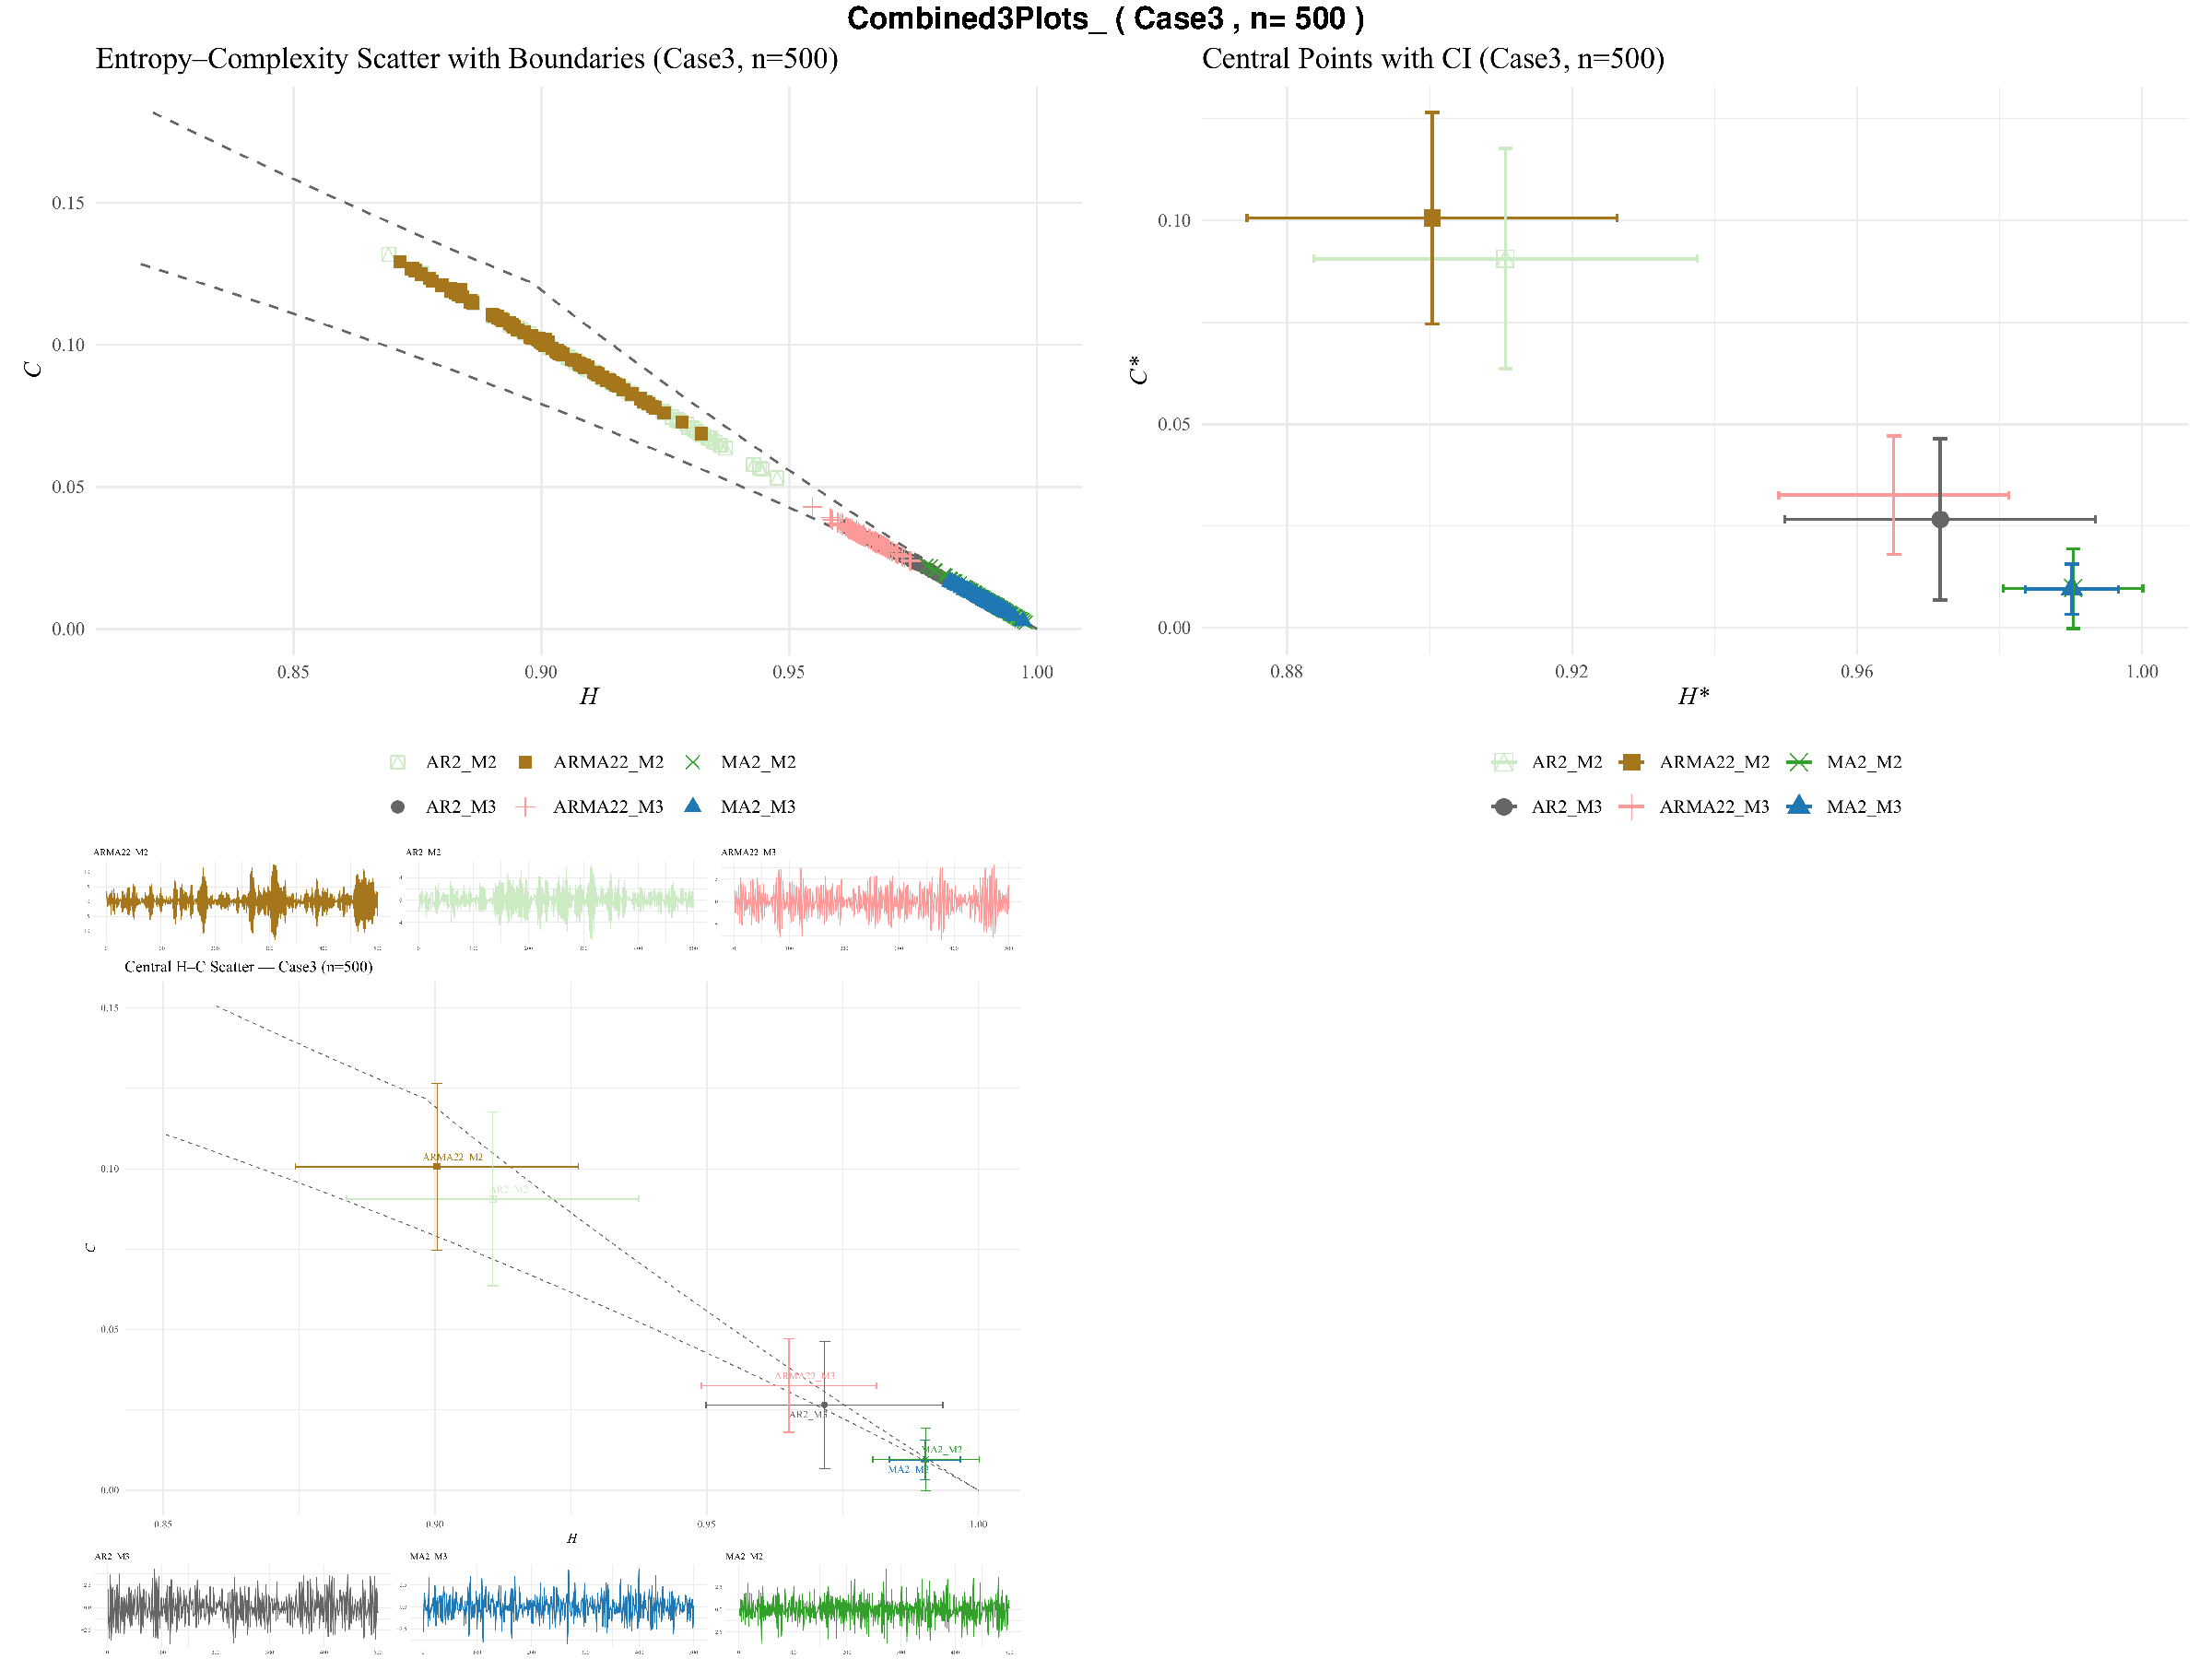
\includegraphics[width=\textwidth]{Combined3Plots_Case3_n500.pdf}
		\captionof{figure}{Entropy–complexity scatter plot and associated time series ($n=500$) for mixed-sign coefficients.}
		\column{0.48\textwidth}
		\centering
		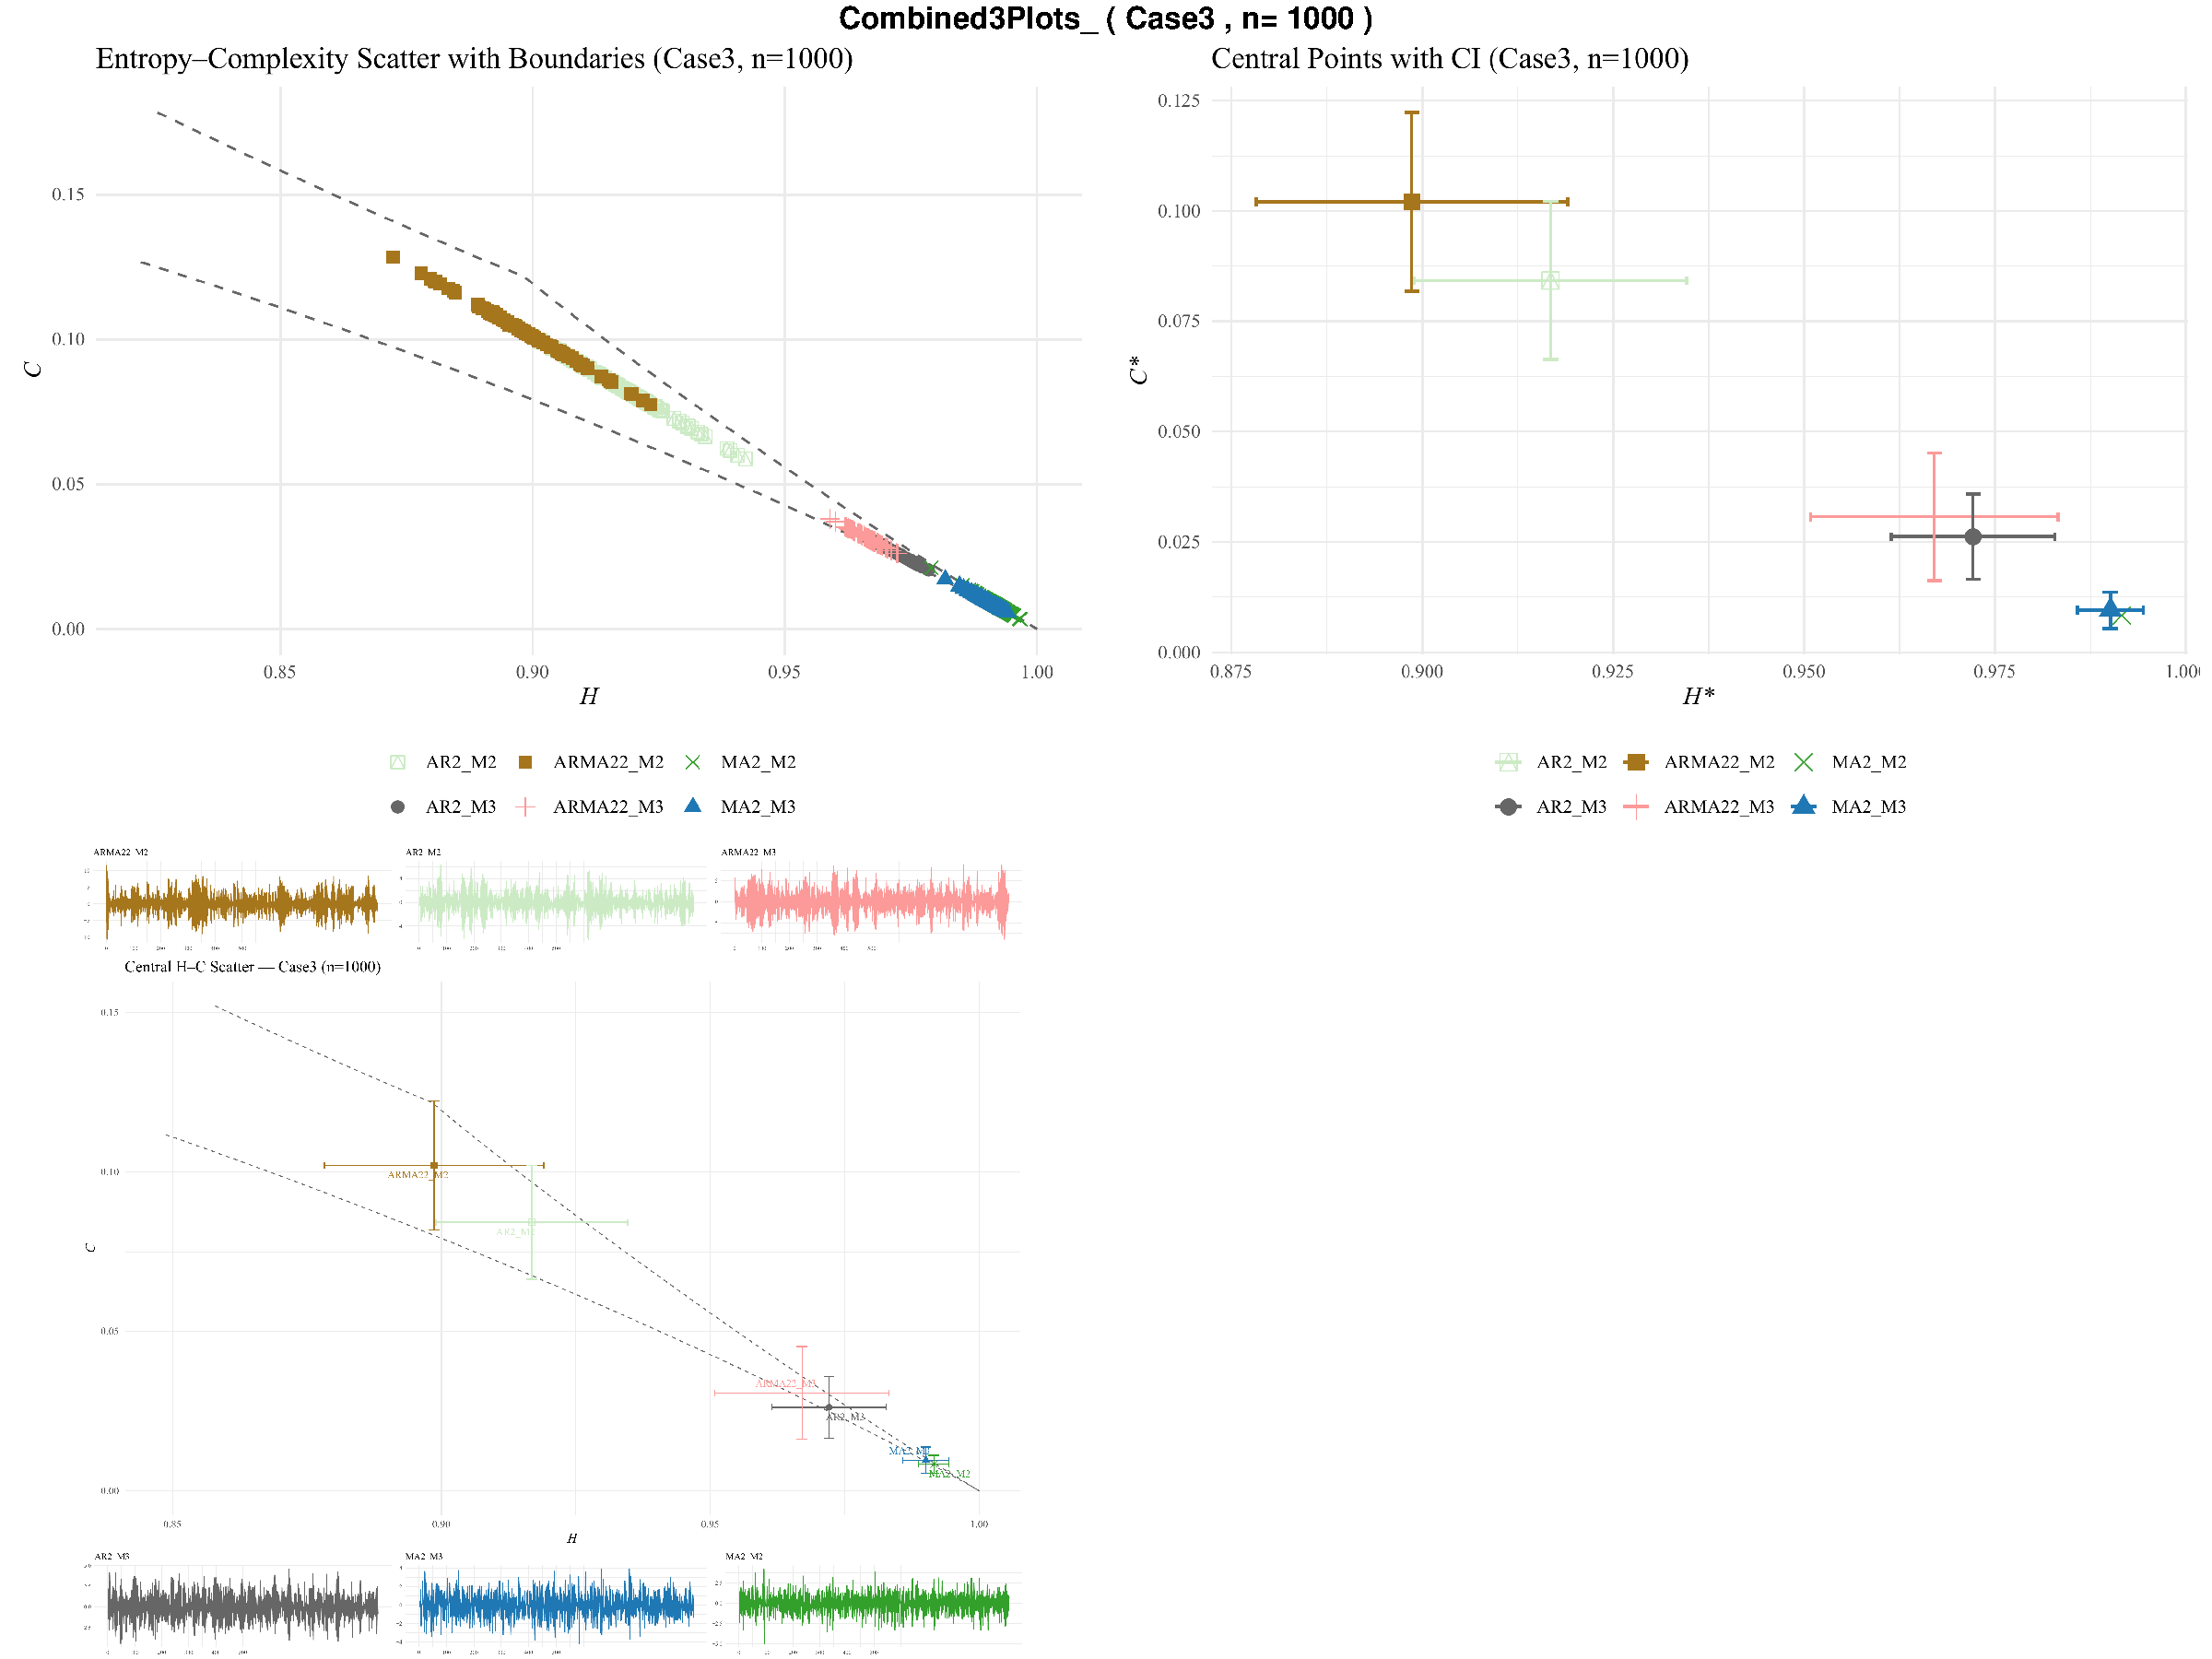
\includegraphics[width=\textwidth]{Combined3Plots_Case3_n1000.pdf}
		\captionof{figure}{Entropy–complexity scatter plot and associated time series ($n=1000$) for mixed-sign coefficients.}
	\end{columns}
\end{frame}

	
	%-----------------------------------------------------%
	\begin{frame}{Extended Cases}
		\begin{itemize}
			\item Focused on three ARMA configurations:
			\begin{itemize}
				\item Two extremes far apart in the $H–C$ plane
				\item One central (median) model
			\end{itemize}
			\item Generated 100 replications for $n=500$ and $n=1000$.
			\item Permutation entropy used for all extended analyses.
		\end{itemize}
		\begin{columns}[c]
			\column{0.48\textwidth}
			\centering
			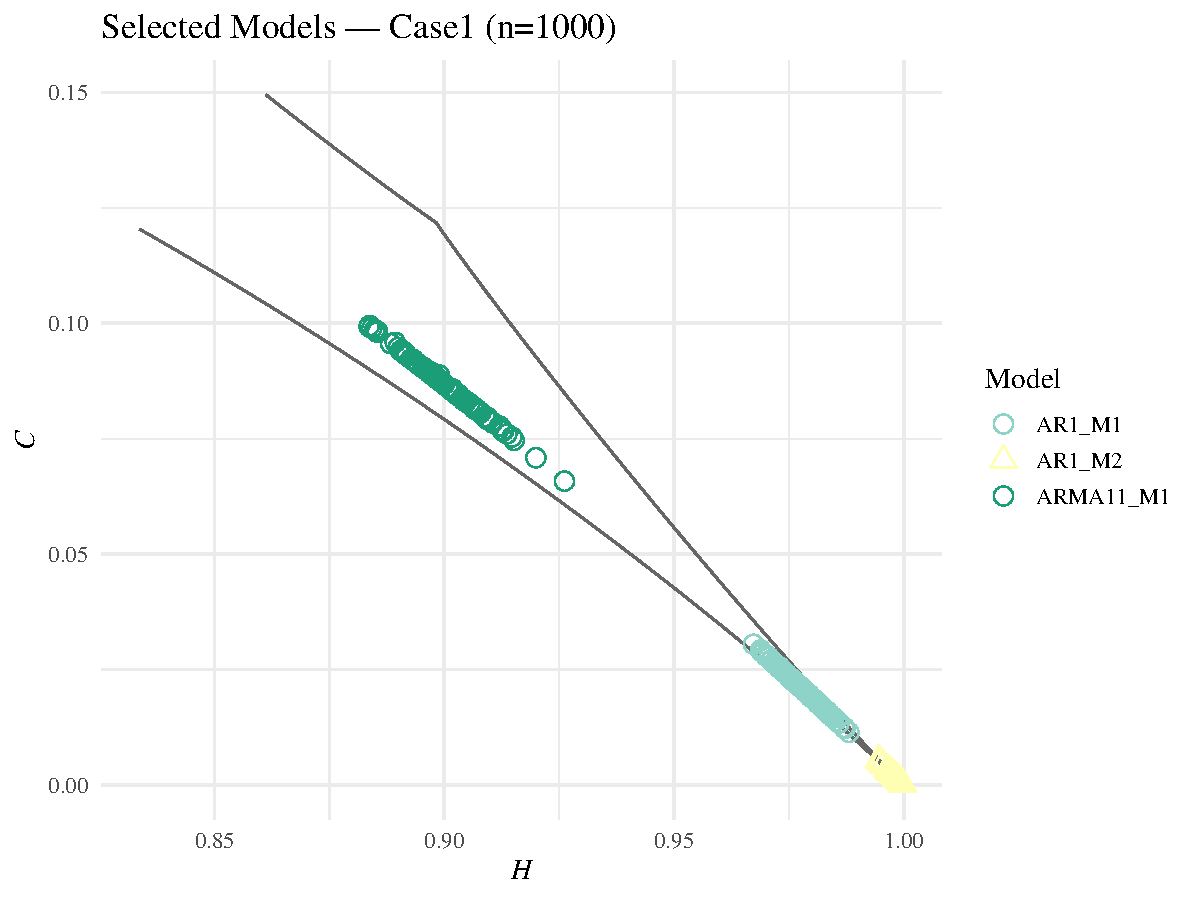
\includegraphics[width=\textwidth]{Scatter_Selected_Case1_n1000.pdf}
			\captionof{figure}{Scatter plot for selected models in the entropy–complexity plane for Case 1.}
			\column{0.48\textwidth}
			\centering
			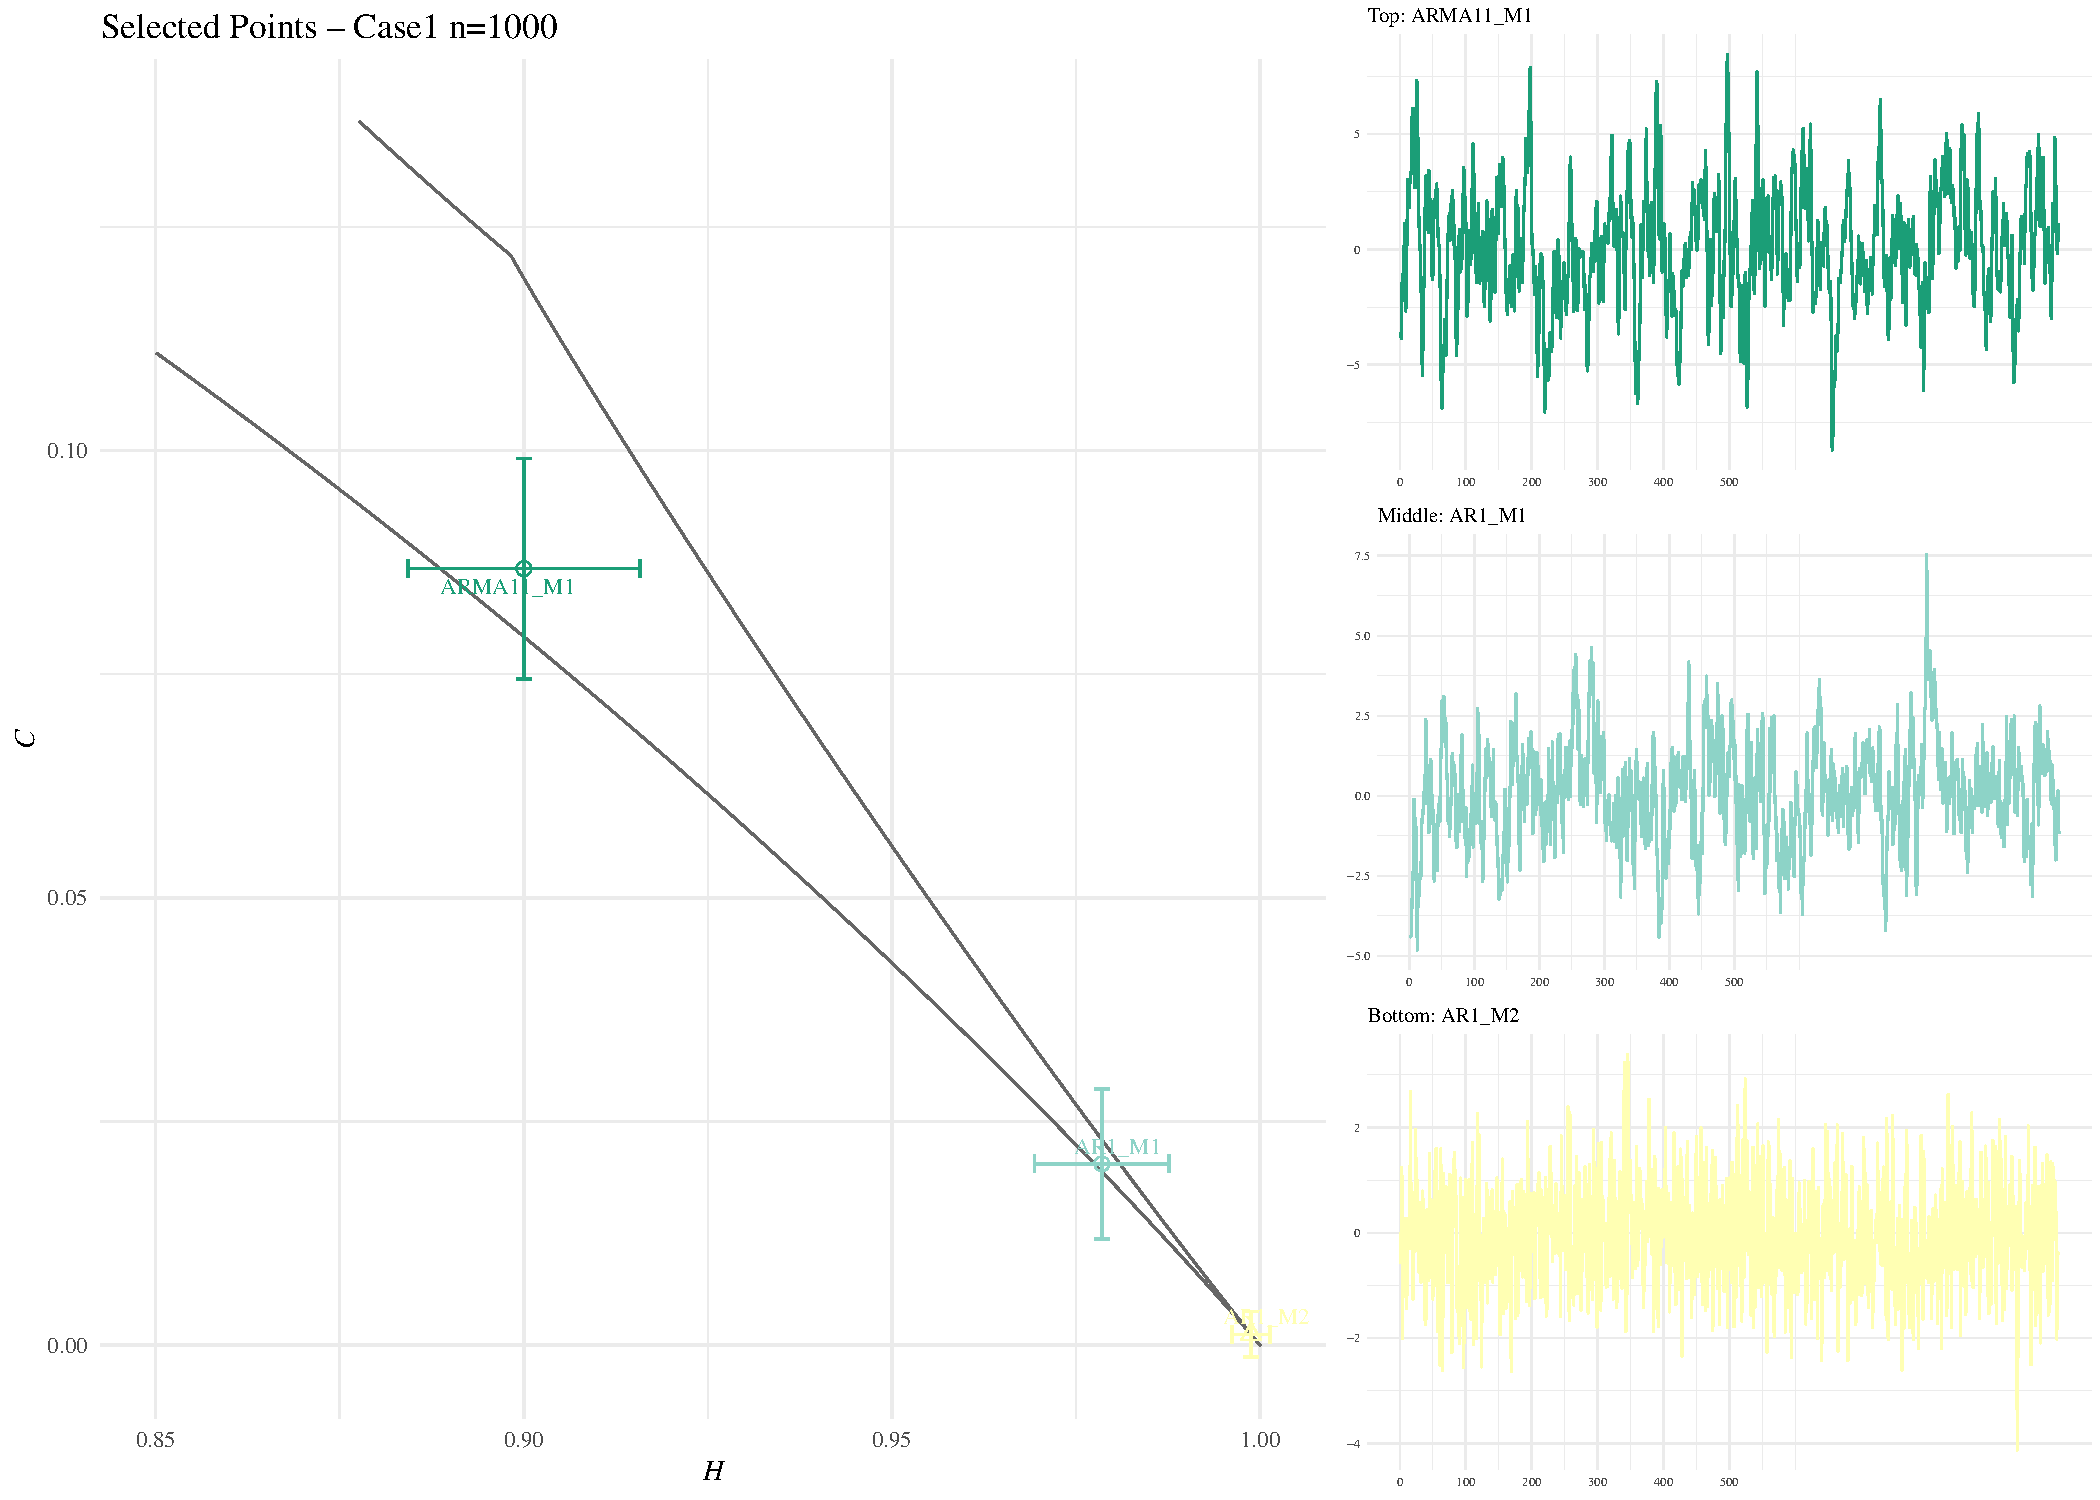
\includegraphics[width=\textwidth]{new_centralpoint_timeseries_Case1_n1000.pdf}
			\captionof{figure}{Representative time series around their central $(H^*, C^*)$ points.}
		\end{columns}
	%	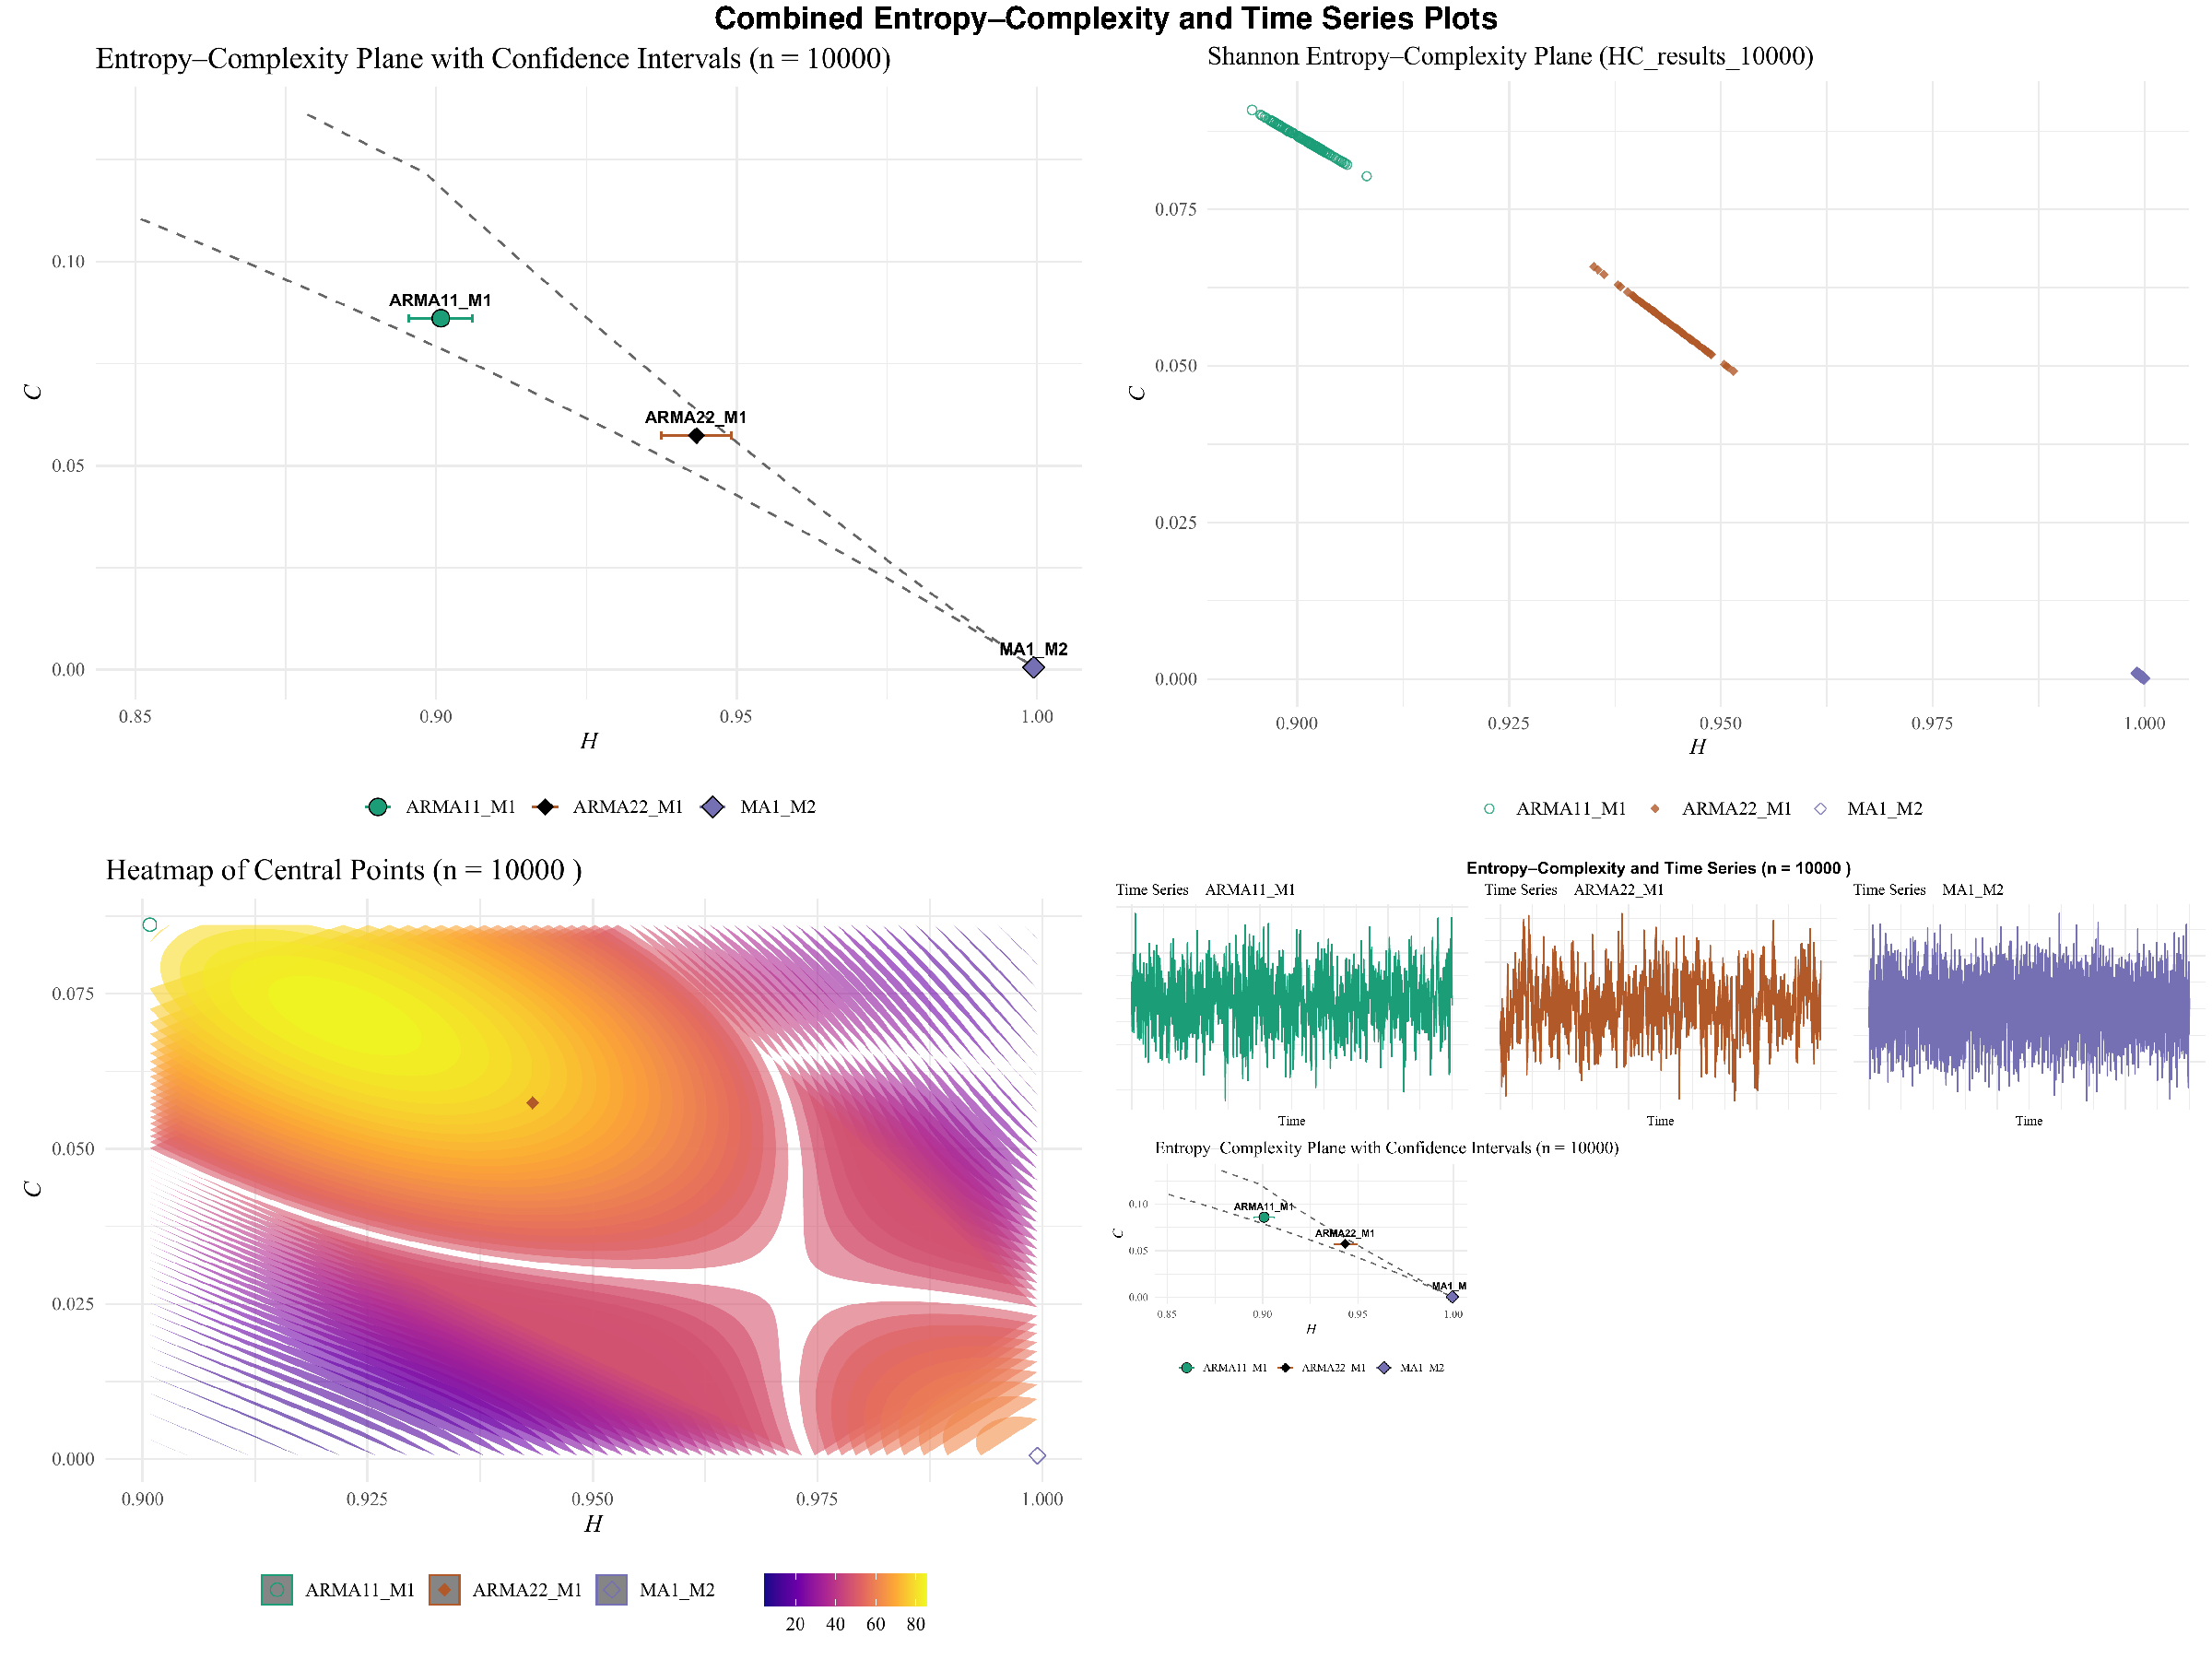
\includegraphics[width=0.6\textwidth]{Combined_4Plots_Case4_n10000.pdf}
	\end{frame}
	
	%-----------------------------------------------------%
	\begin{frame}{Extended Cases cont\dots}
		\begin{columns}[c]
			\column{0.48\textwidth}
			\centering
			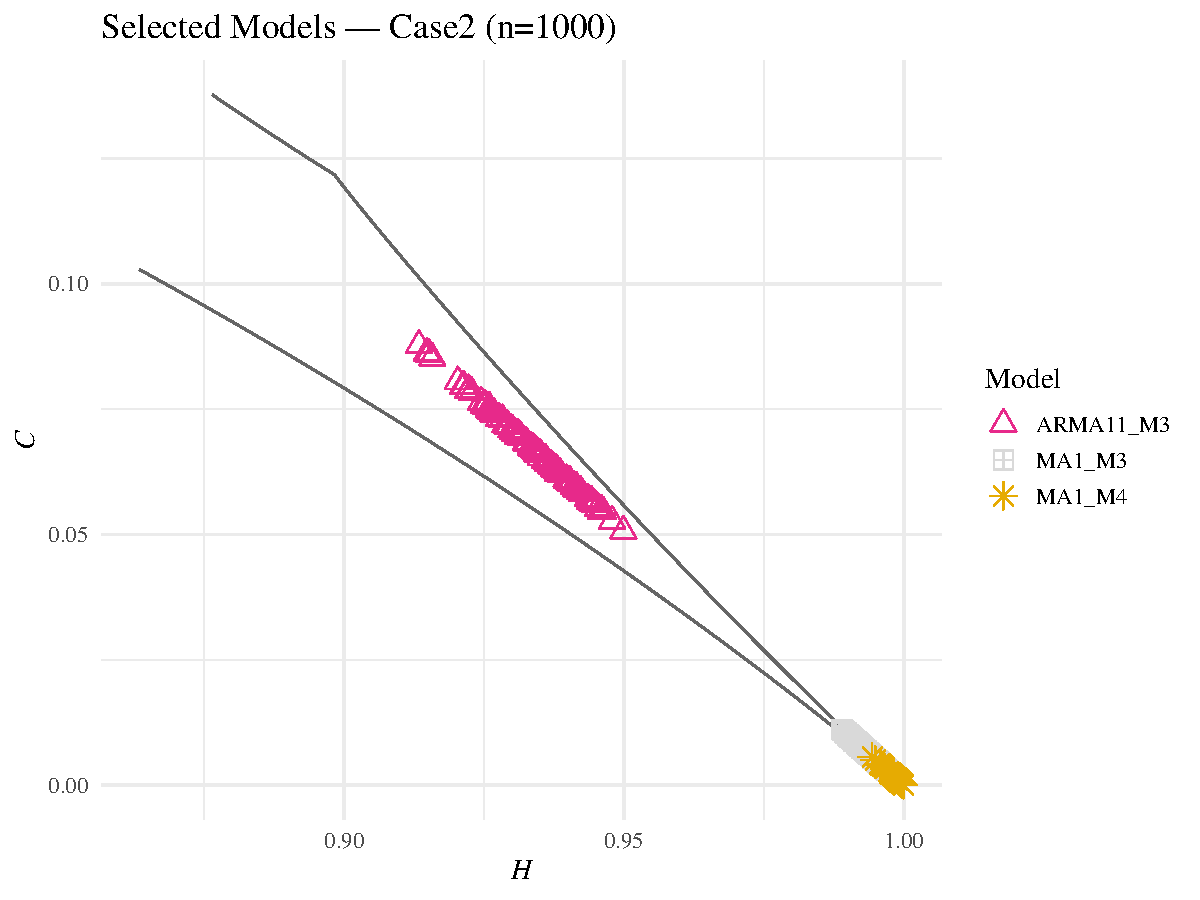
\includegraphics[width=\textwidth]{Scatter_Selected_Case2_n1000.pdf}
			\captionof{figure}{Scatter plot for selected models in the entropy–complexity plane for Case 2.}
			\column{0.48\textwidth}
			\centering
			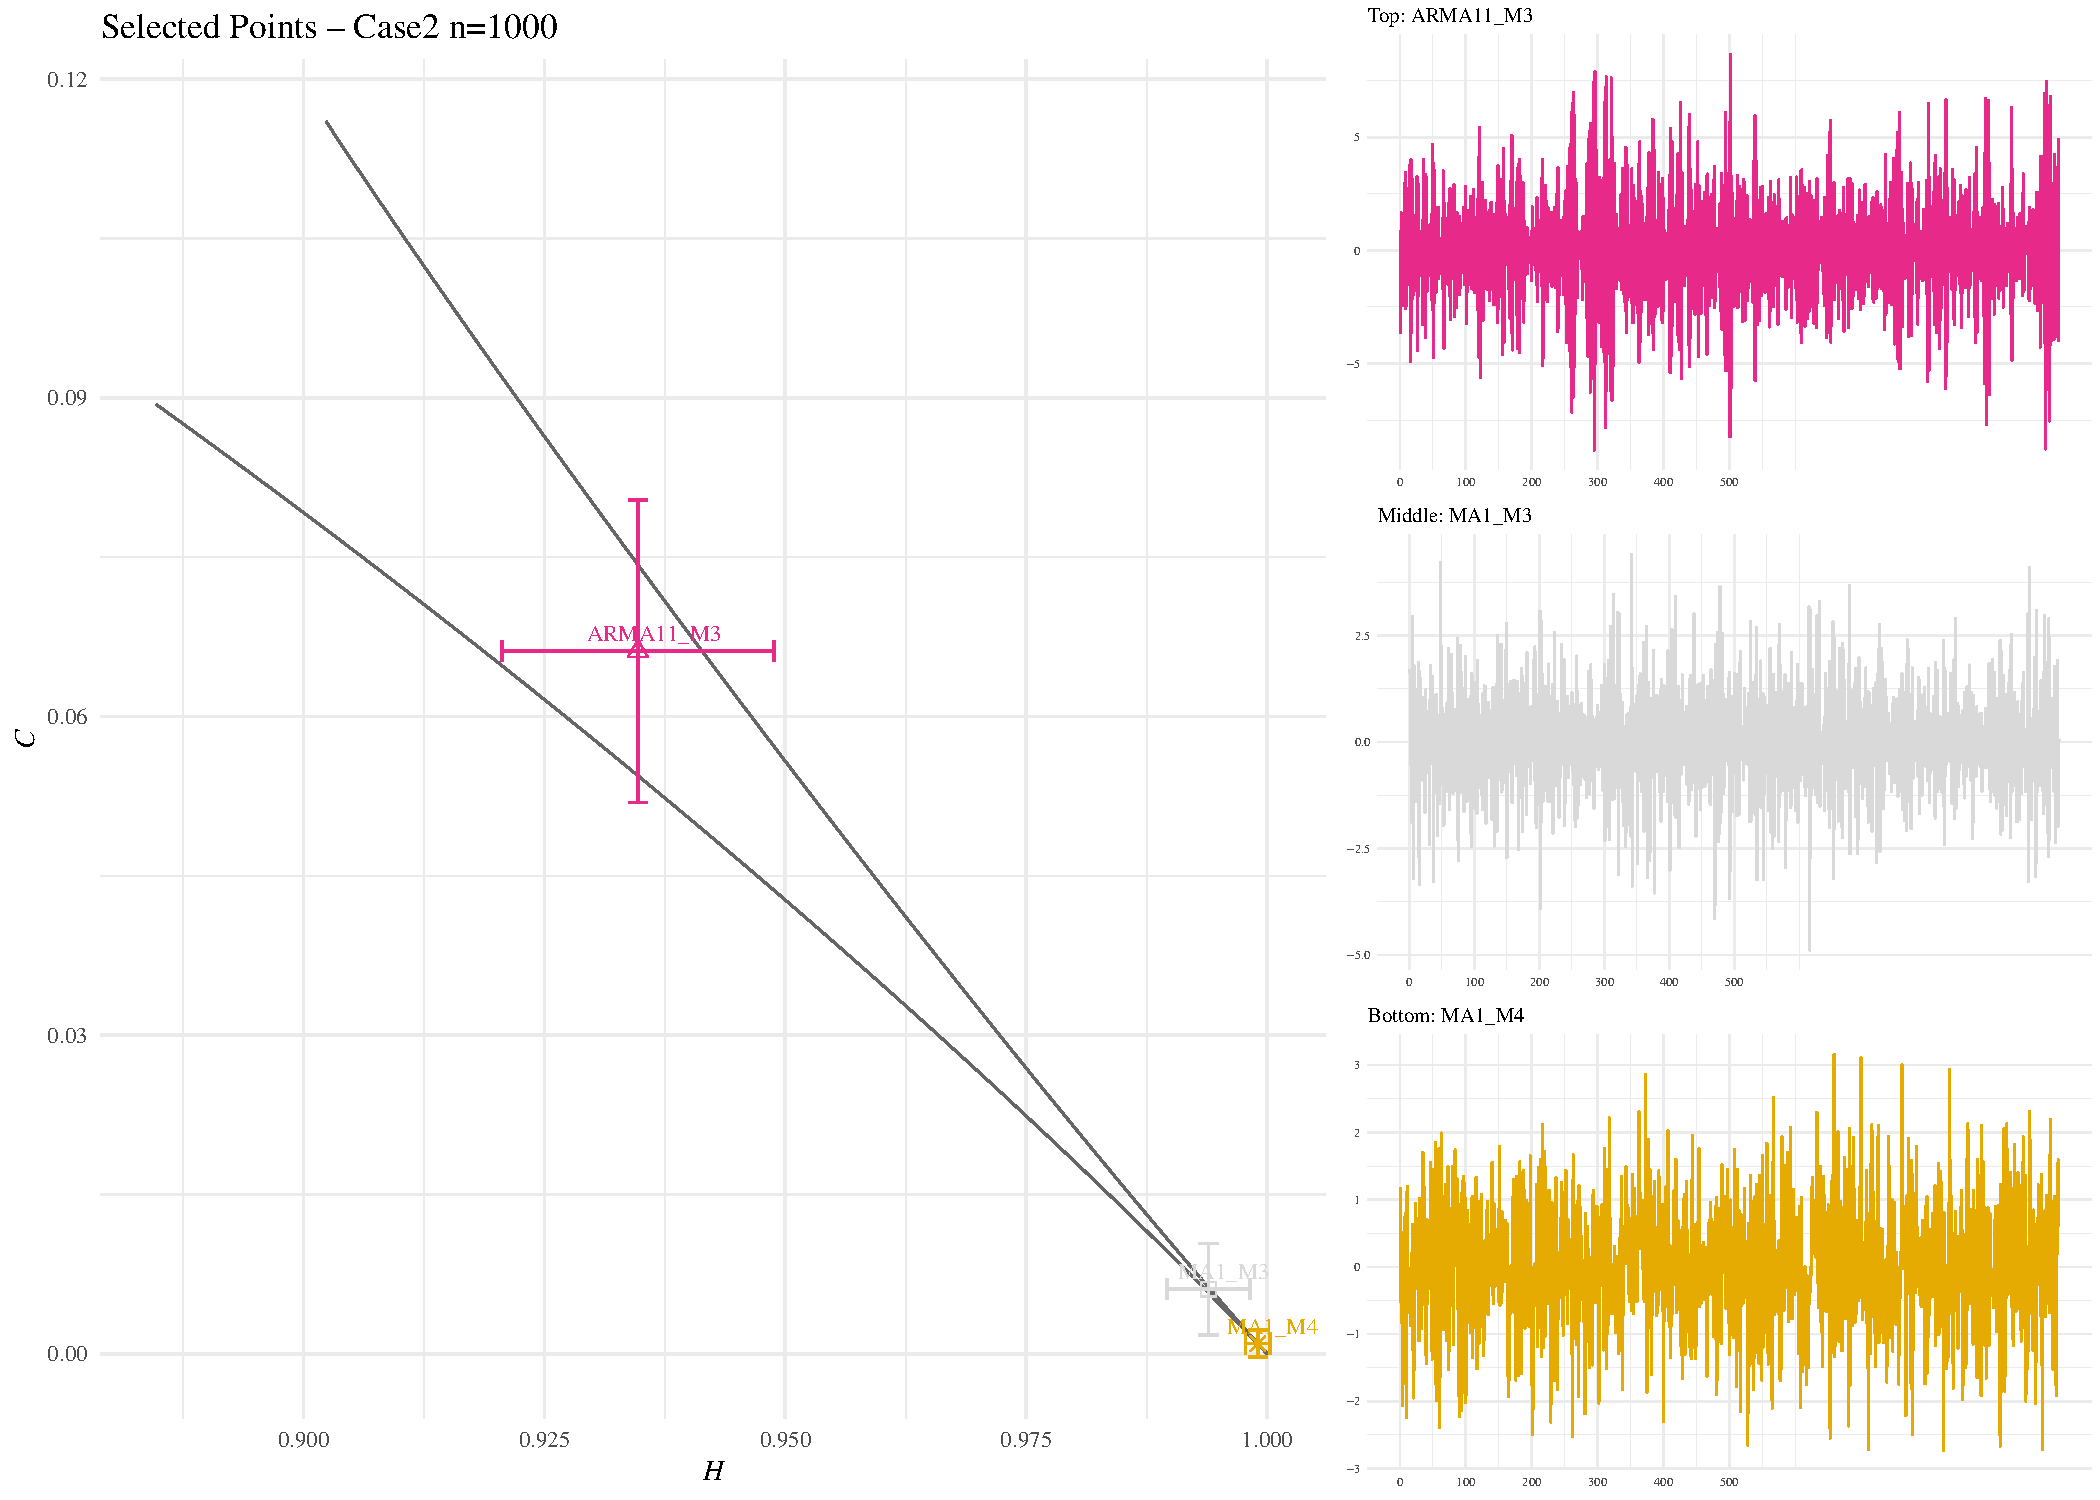
\includegraphics[width=\textwidth]{new_centralpoint_timeseries_Case2_n1000.pdf}
			\captionof{figure}{Representative time series around their central $(H^*, C^*)$ points.}
		\end{columns}
	\end{frame}
	
	%-----------------------------------------------------%
	\begin{frame}{Extended Cases cont\dots}
		\begin{columns}[c]
			\column{0.48\textwidth}
			\centering
			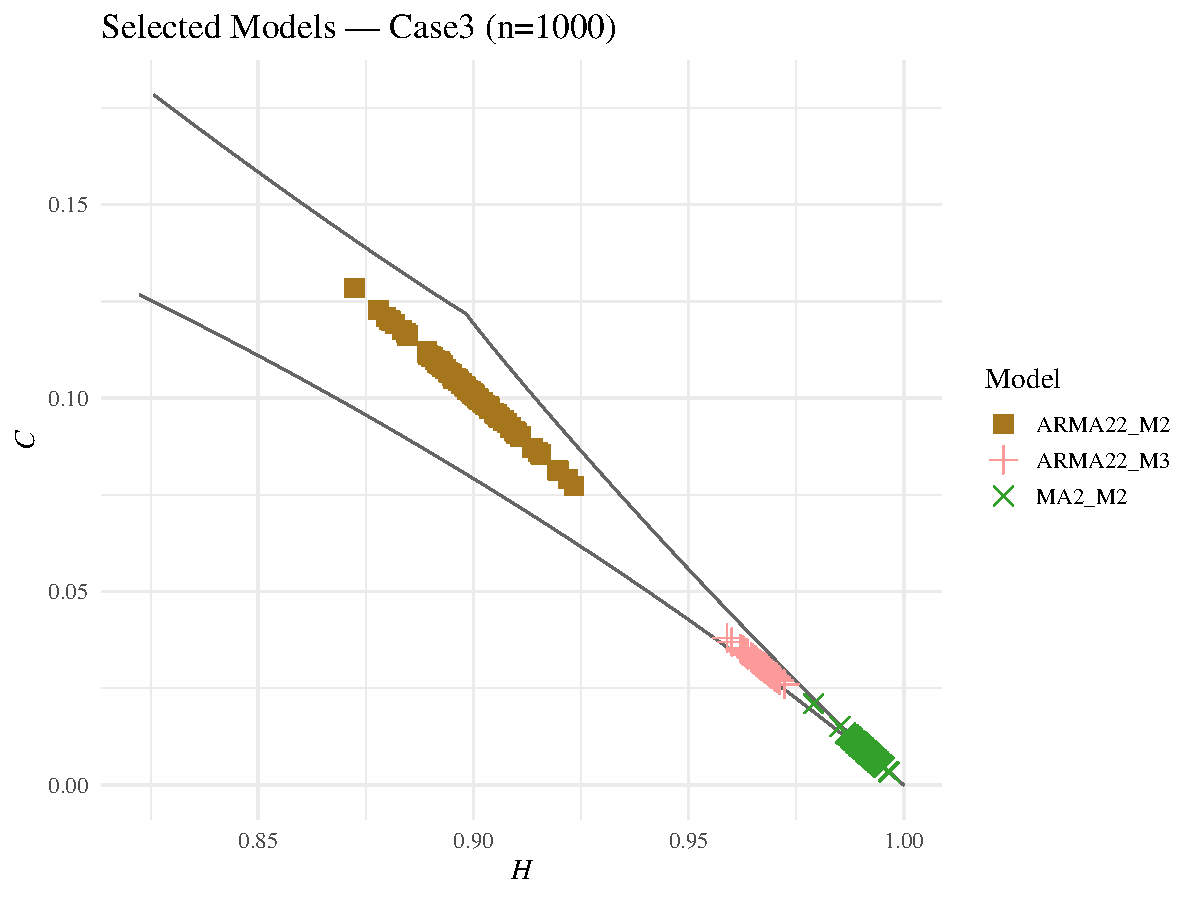
\includegraphics[width=\textwidth]{Scatter_Selected_Case3_n1000.pdf}
			\captionof{figure}{Scatter plot for selected models in the entropy–complexity plane for Case 3.}
			\column{0.48\textwidth}
			\centering
			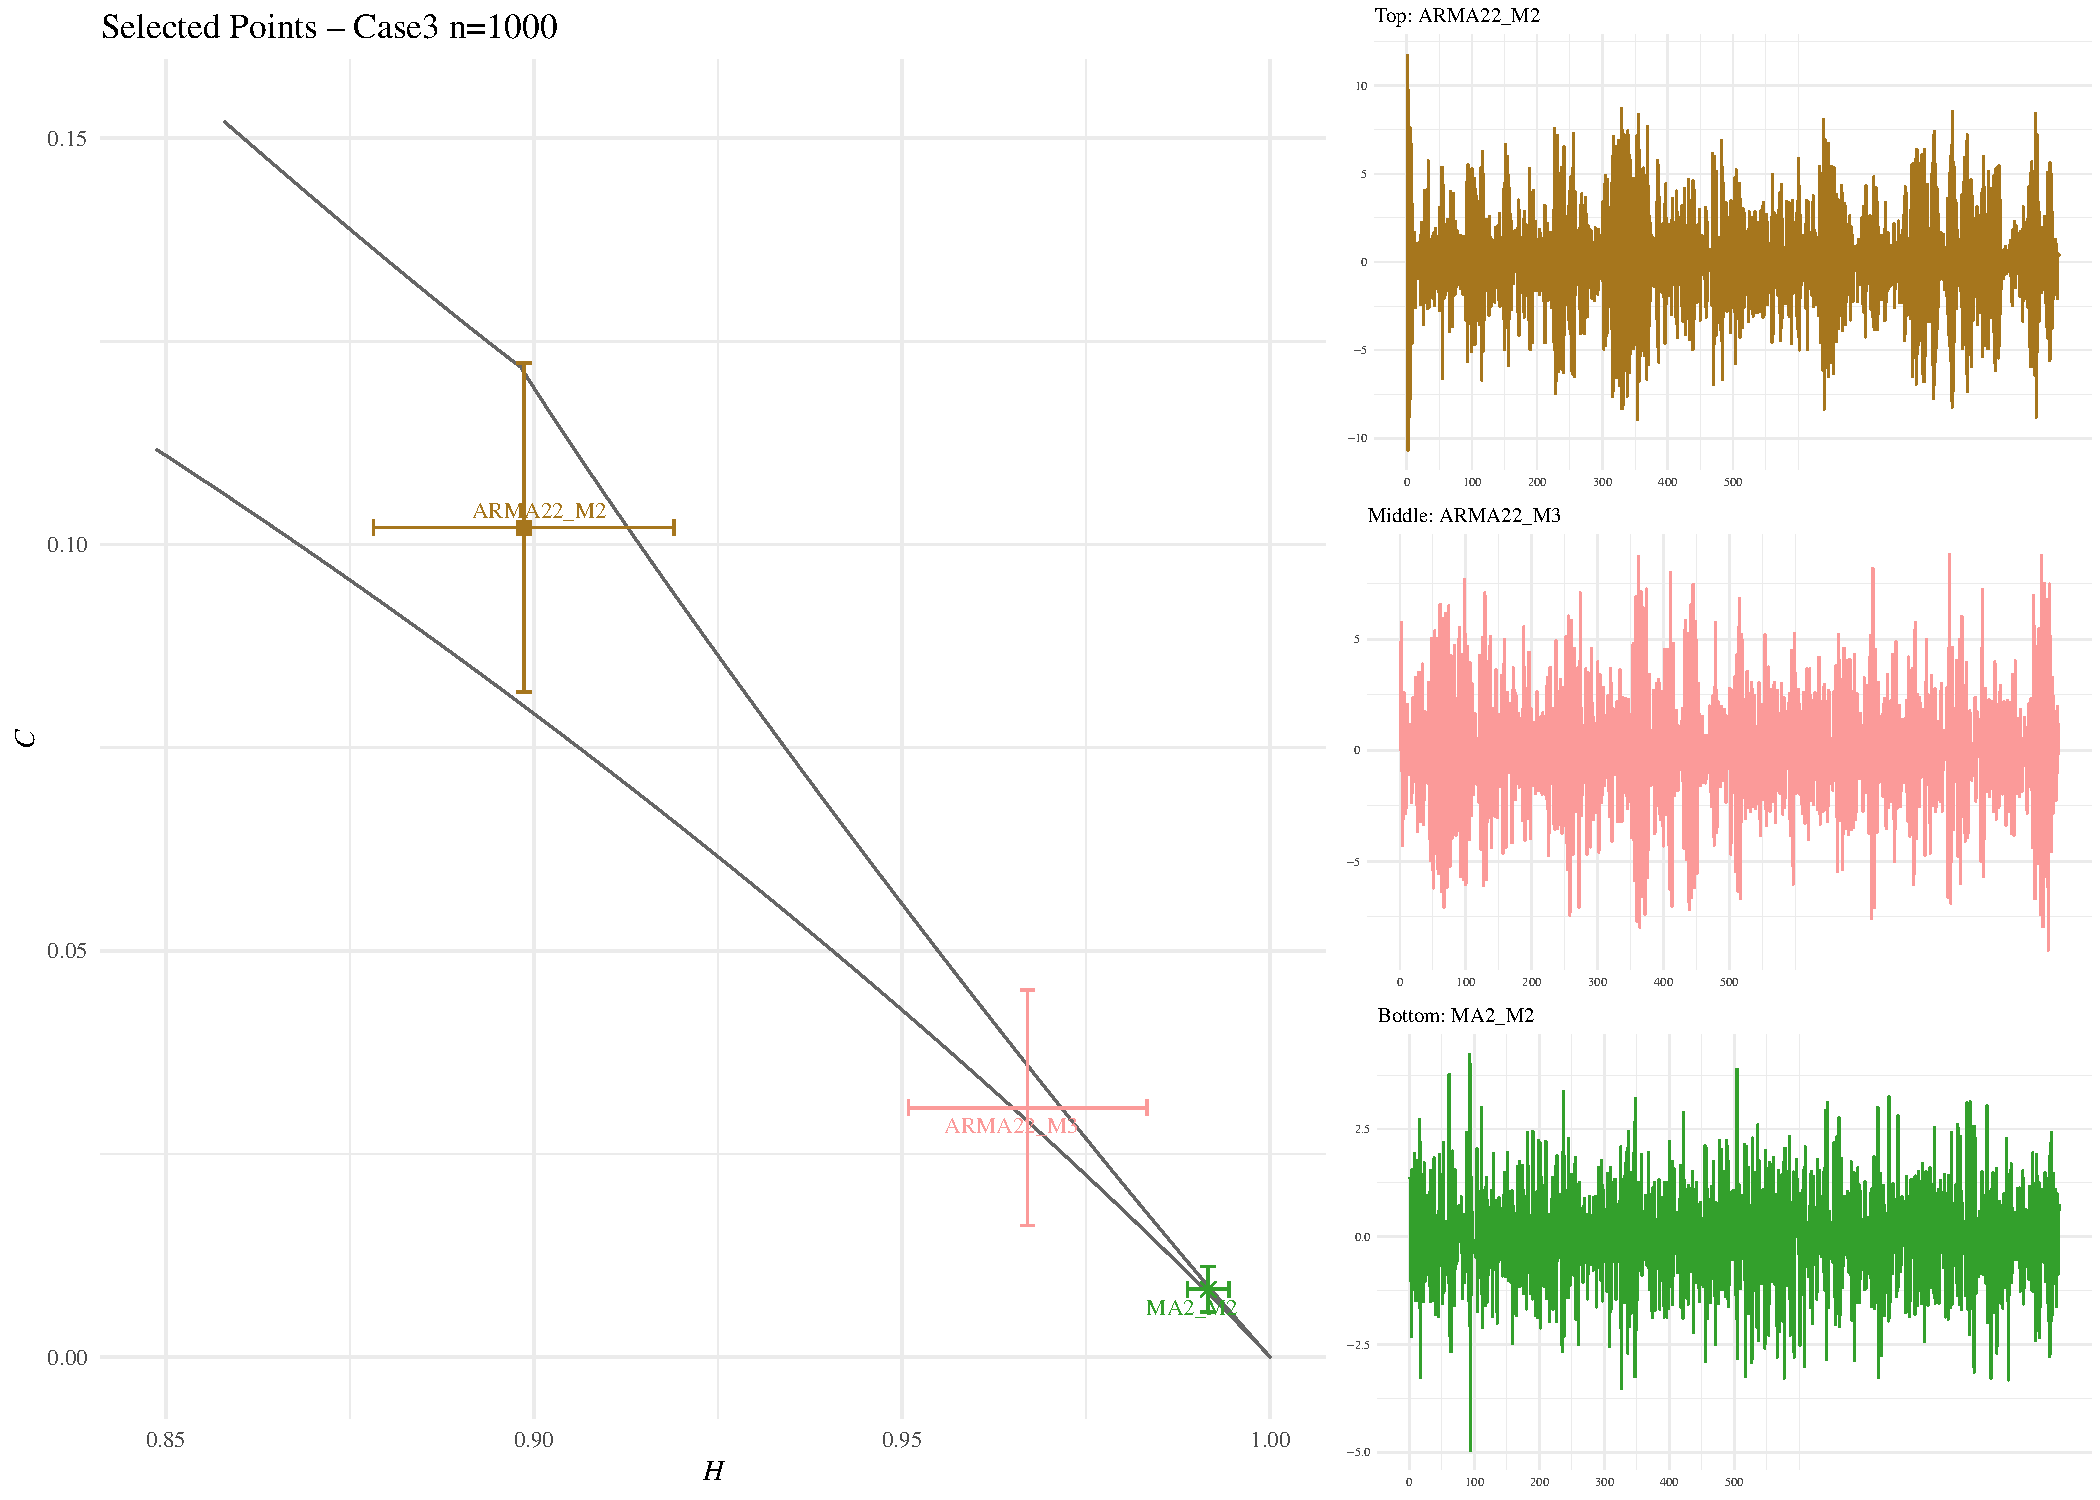
\includegraphics[width=\textwidth]{new_centralpoint_timeseries_Case3_n1000.pdf}
			\captionof{figure}{Representative time series around their central $(H^*, C^*)$ points.}
		\end{columns}
	\end{frame}
	
	%===========================================================
\section{Combined Model Visualization}
\begin{frame}{All Models and Patterns}
		\centering
		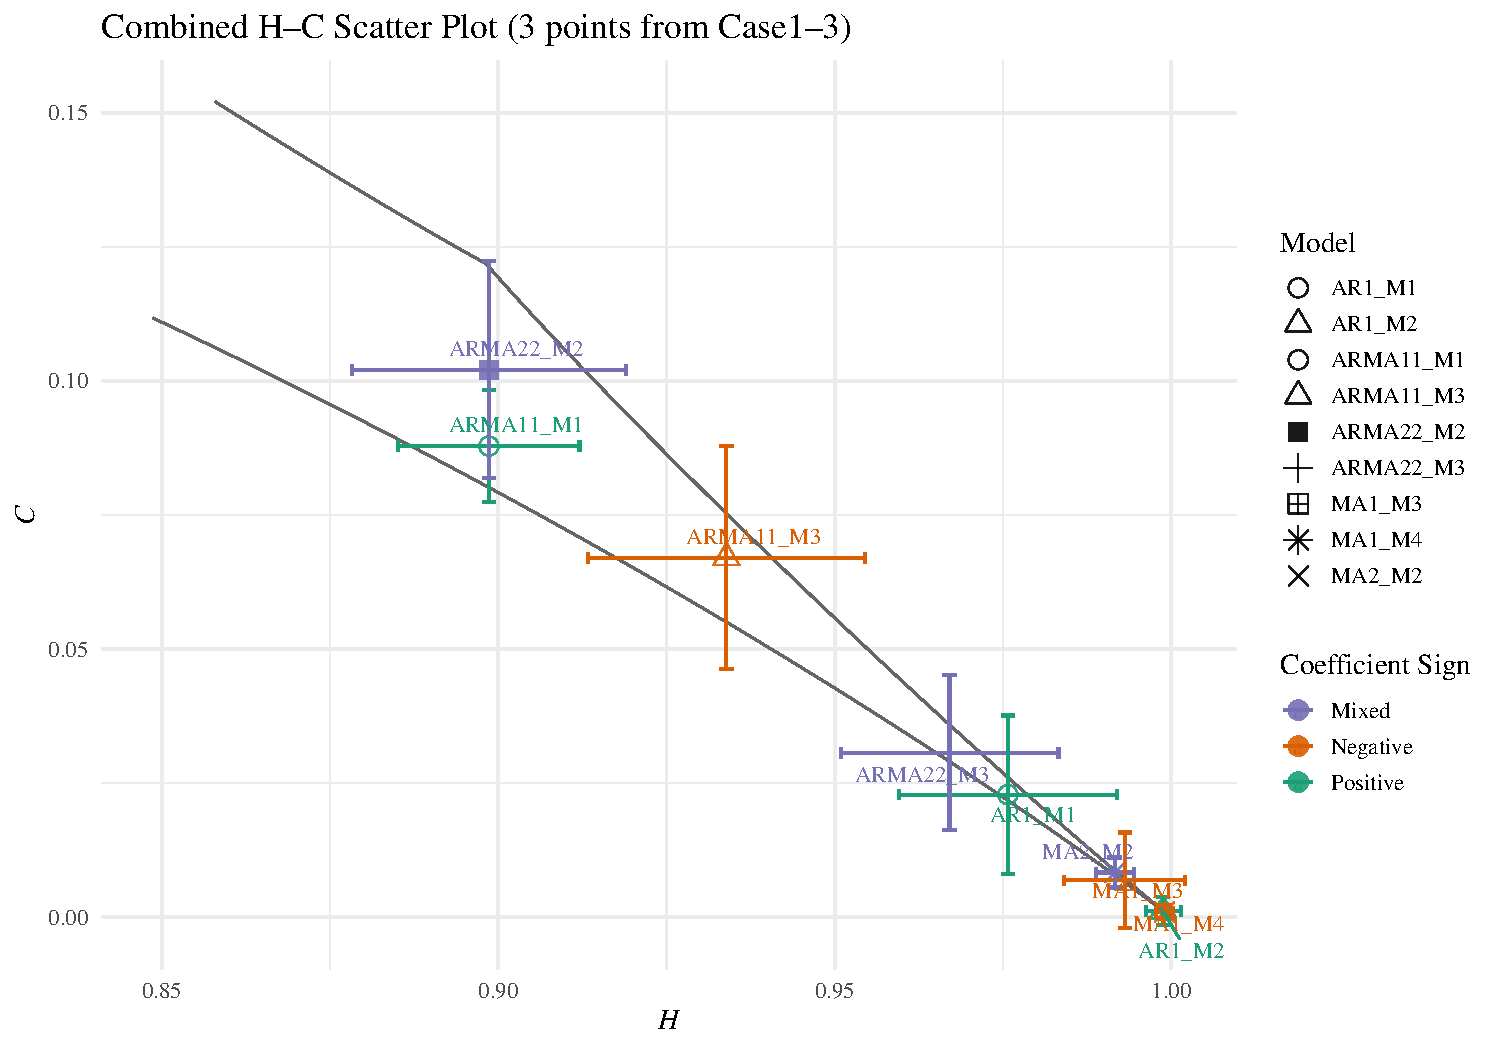
\includegraphics[width=\textwidth]{combined_new_scatterplot.pdf}
		\captionof{figure}{All models combined in the entropy–complexity plane.}
		\centering
	\end{frame}

	
	%===========================================================
	\section{Summary and Conclusion}
	\begin{frame}{Key Findings}
		\begin{itemize}
			\item Ordinal pattern analysis successfully distinguishes AR, MA, and ARMA models.
			\item Distinct clustering appears across Permutation entropy.
			\item Central $(H^*, C^*)$ points provide consistent model representation.
			\item Larger samples yield tighter clusters and improved discrimination.
		\end{itemize}
	\end{frame}
	
	%-----------------------------------------------------%
	\begin{frame}{Conclusion}
		\begin{block}{Summary}
			This study reveals that combining ordinal pattern analysis with entropy–complexity measures provides a robust framework for model discrimination in simulated time series.
		\end{block}
		\begin{itemize}
			\item Captures both linear and nonlinear relationship between the entropy and complexity.
			\item Overlap points reveal intrinsic similarities in model dynamics.
			\item Extensible to real-world applications such as finance, engineering, biomedical signals.
		\end{itemize}
	\end{frame}
	
	%-----------------------------------------------------%
	\begin{frame}{Future Work}
		\begin{itemize}
			\item Apply unsupervised clustering (e.g., k-means, hierarchical) in the $H–C$ plane.
			\item Extend analysis by increasing sample size
			\item Extend distinct clustering using other types of entropies Rényi, Tsallis, and Fisher Information. 
			\item Extend analysis to empirical systems.
		\end{itemize}
	\end{frame}
	
	%-----------------------------------------------------%
	\begin{frame}[plain]
		\centering
		\Huge \textbf{Thank You!} \\
		\vspace{0.5cm}
		\small Contact: \href{mailto:rasika.dilhani@vuw.ac.nz}{rasika.dilhani@vuw.ac.nz}
	\end{frame}
	
	%-----------------------------------------------------%
	\begin{frame}[allowframebreaks]{References}
		\bibliographystyle{alpha}
		\bibliography{../../../BearingFaultDiagnosis}
		
	\end{frame}
\end{document}

